% \appendix
\chapter*{Appendix: List of Figures}


\begin{figure}[!ht]
    \centering
    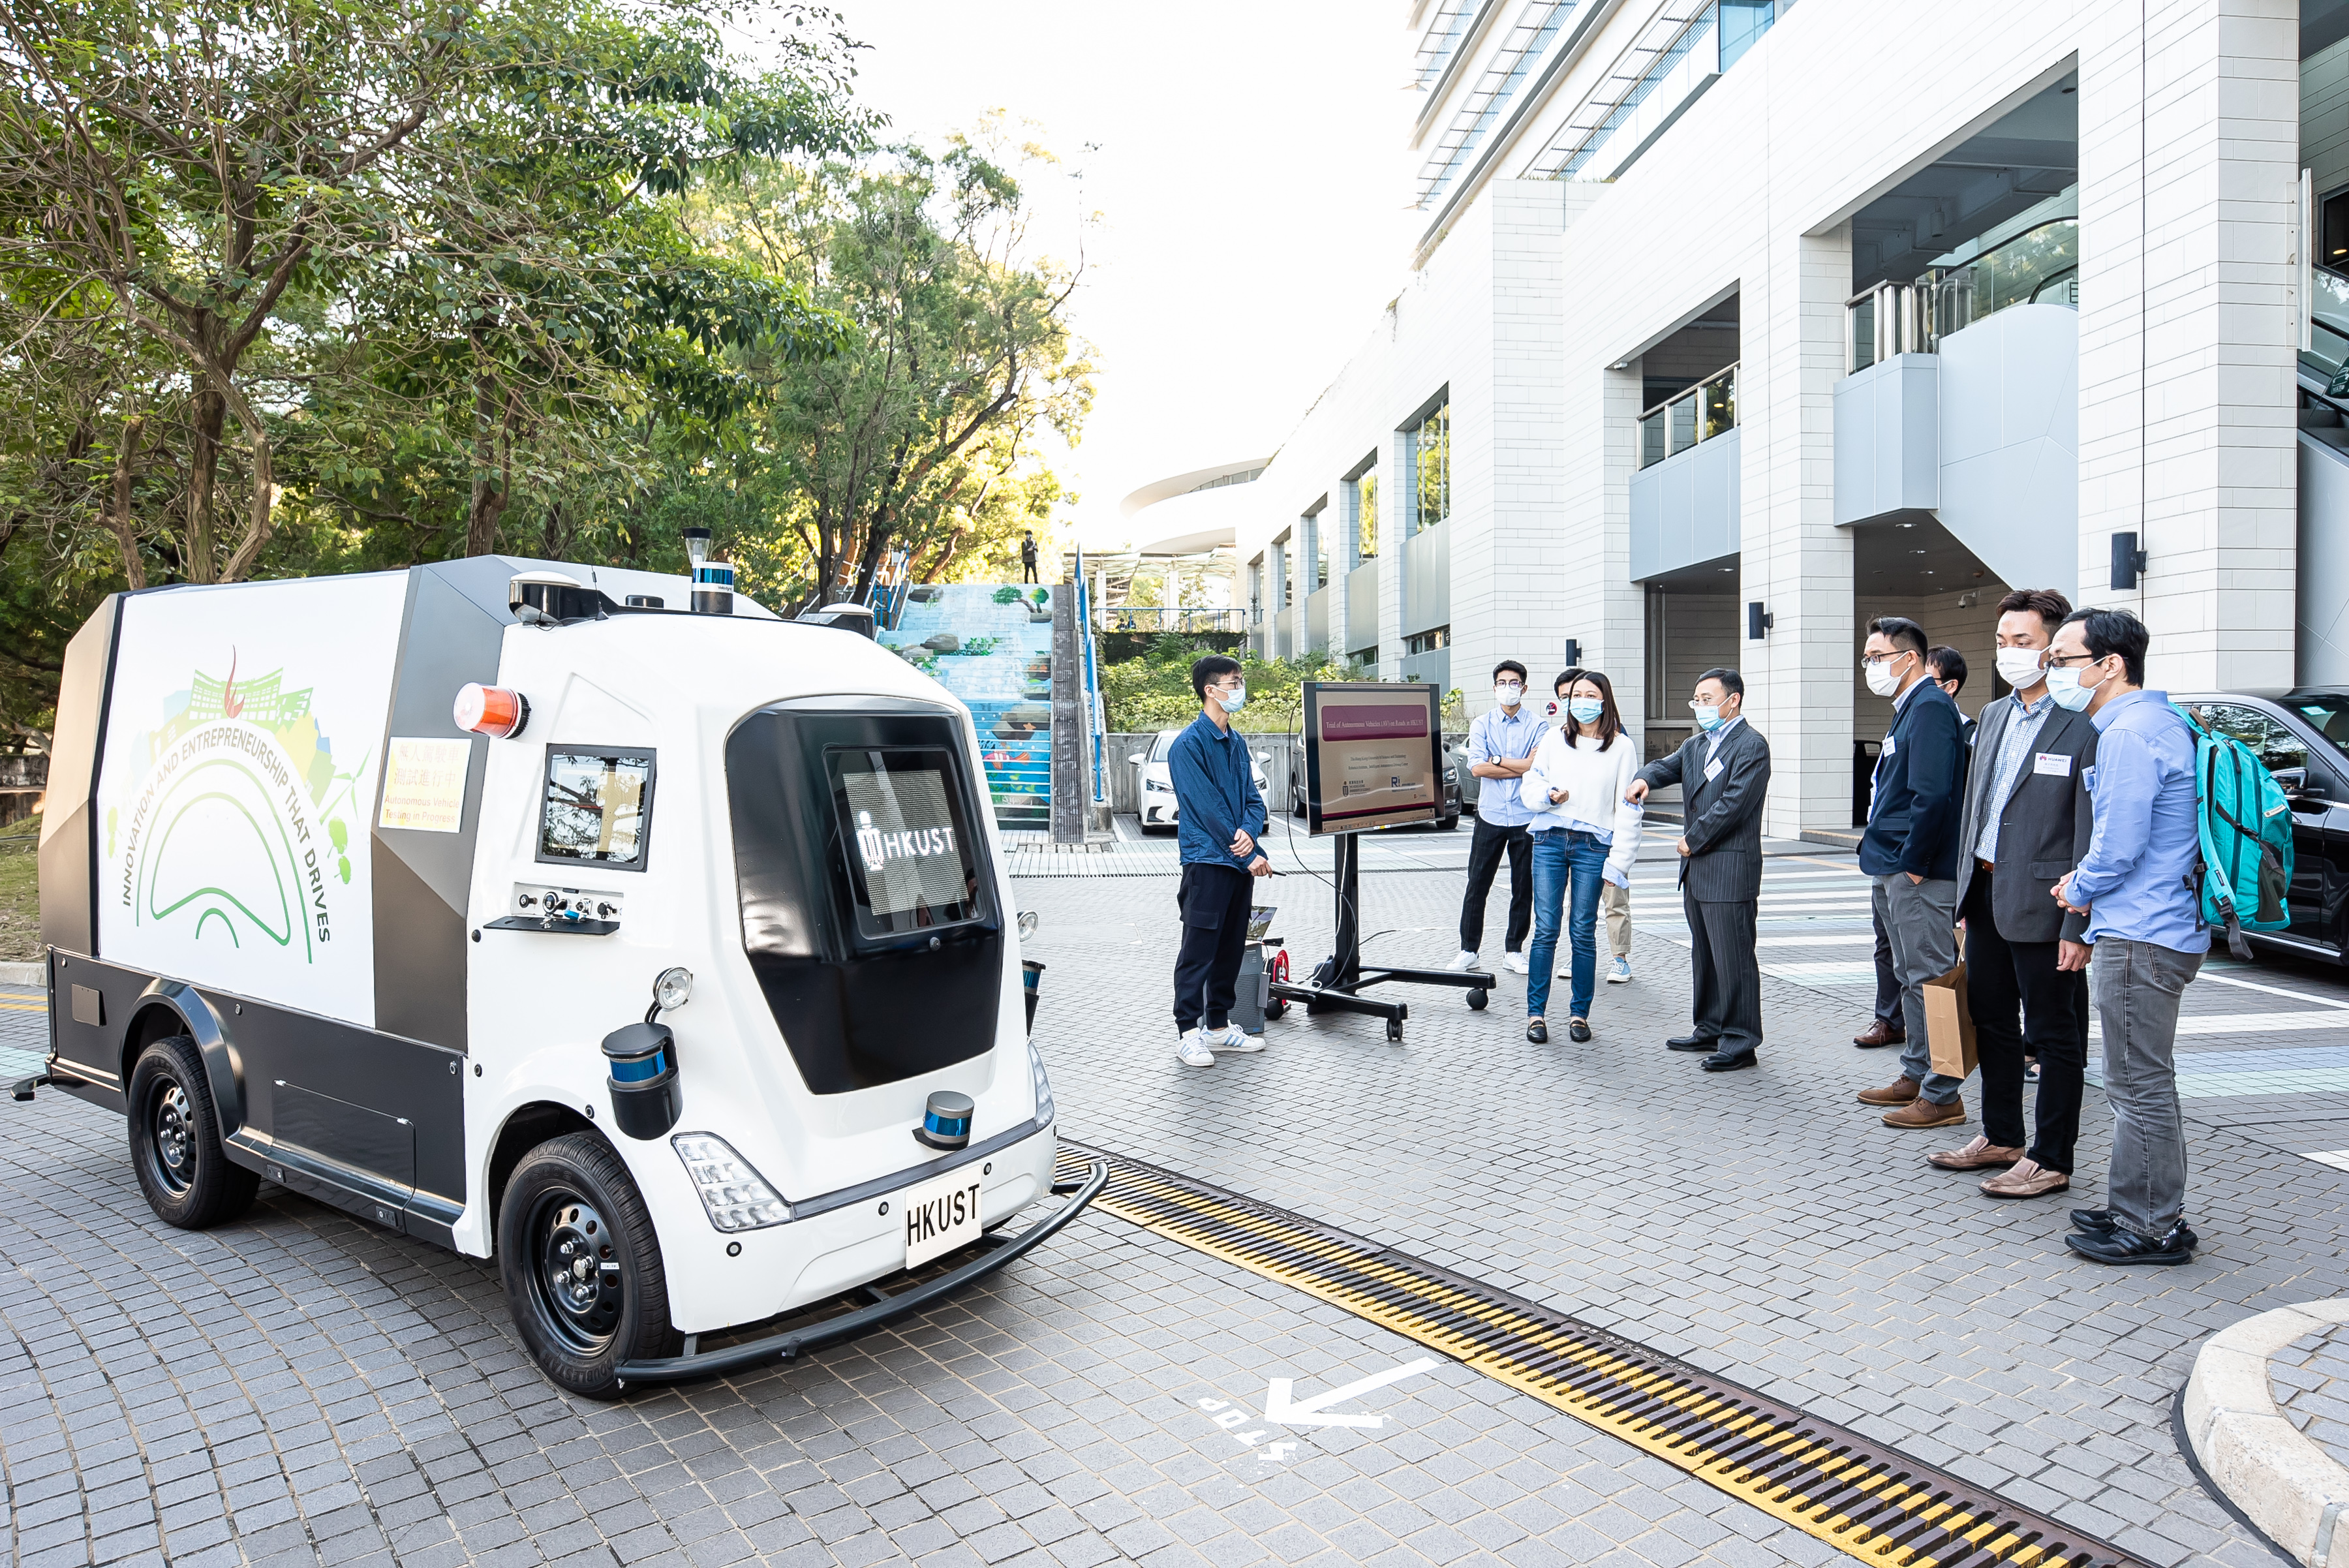
\includegraphics[width=0.9\columnwidth]{figure/pqe/hercules.jpg}
    \caption{The first autonomous vehicle (AV) trial without an operator on board in Hong Kong commenced in late 2020 on the HKUST Clearwater Bay Campus. The AV, designed by Prof. Ming Liu (ECE, Director of HKUST’s Intelligent Autonomous Driving Centre) and his team of students, is one of the many innovative initiatives to fight against the COVID-19 pandemic as the AV can make deliveries that limit human-to-human contact.}
    \label{fig:Hercules}
 \end{figure}

 \begin{figure}[!ht]
    \centering
    \begin{subfigure}{0.45\textwidth}
        \centering
        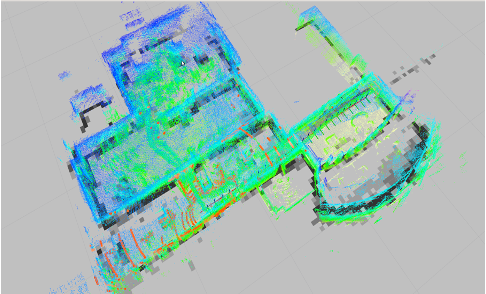
\includegraphics[width=6.5cm, height=4.5cm]{figure/pqe/pointcloudmap.png}
        \caption{A point cloud map of the second floor, HKUST CYT constructed by A-LOAM}
    \end{subfigure}
    \centering
    \begin{subfigure}{0.45\textwidth}
        \centering
        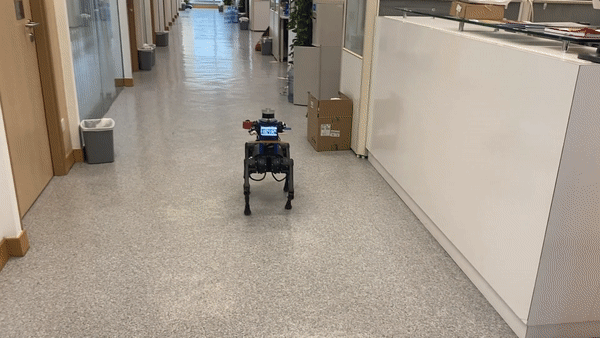
\includegraphics[width=6.5cm, height=4.5cm]{figure/pqe/quadruped.png}
        \caption{A capture of localization on quadruped robot in an indoor office environment.}
    \end{subfigure}
    \caption{Mapping and Localization of Quadruped Robot}
    \label{fig:quadruped}
 \end{figure}

 \begin{figure}[!ht]
    \centering
    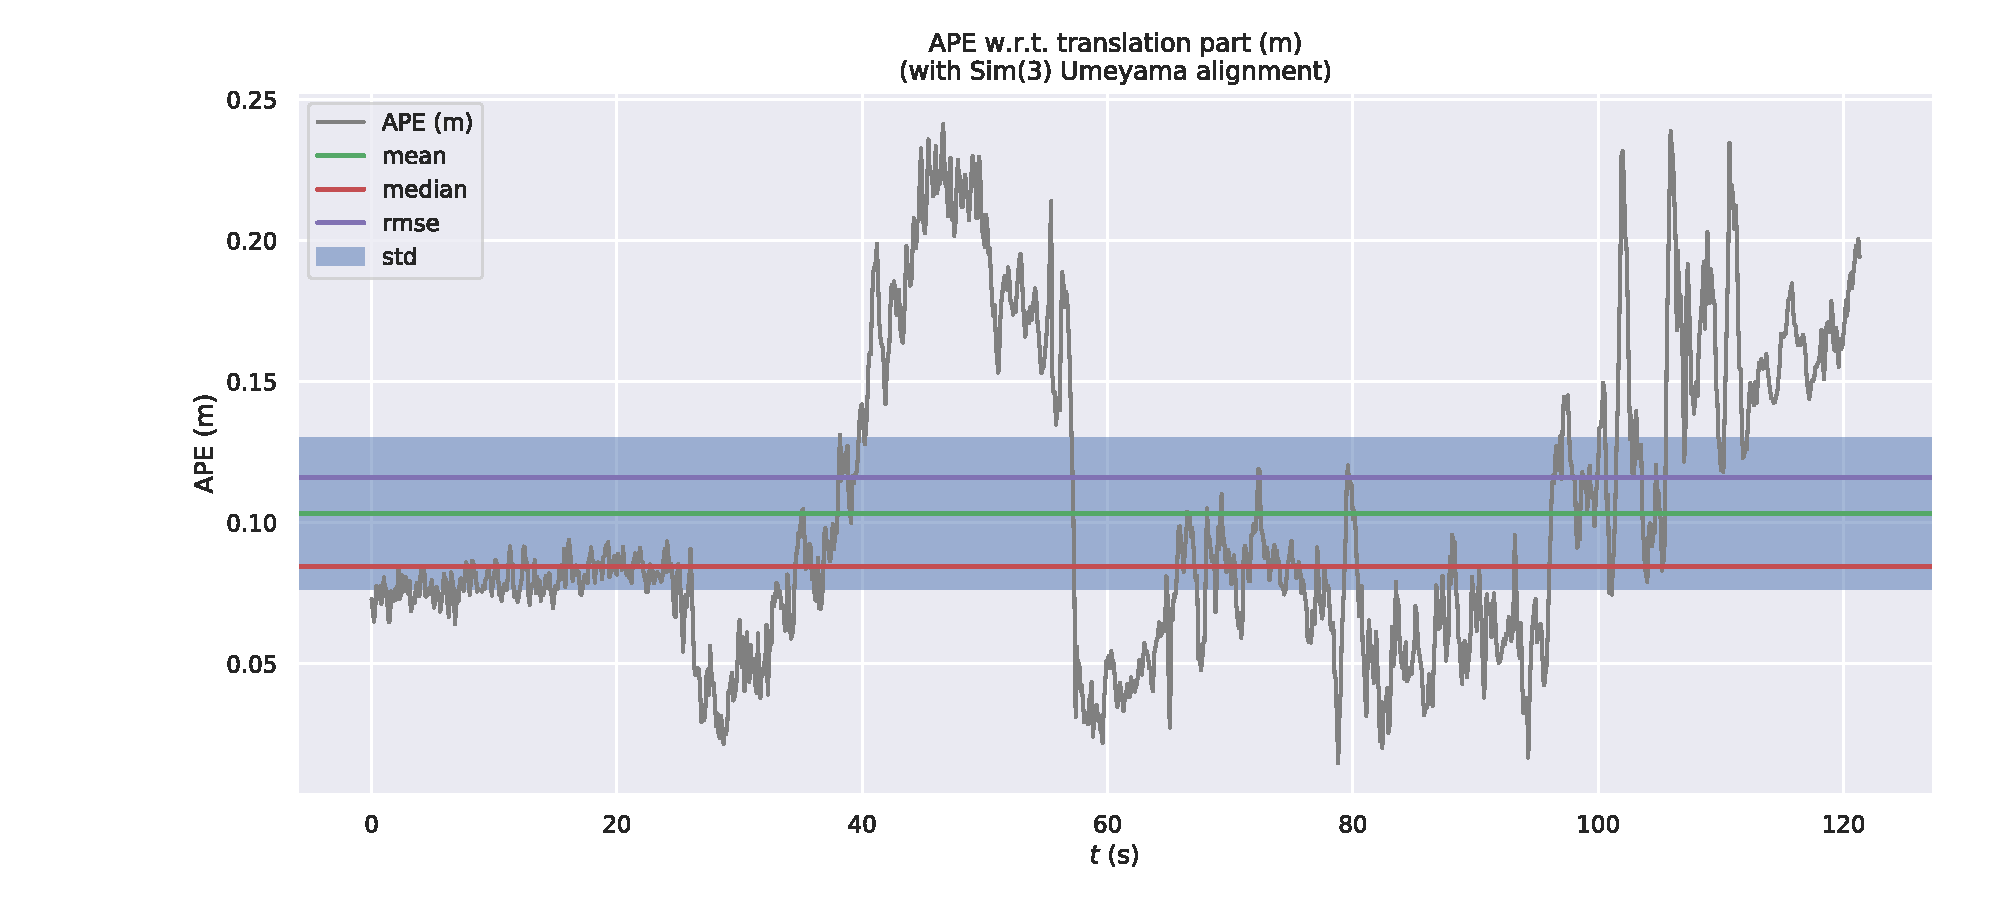
\includegraphics[width=\columnwidth]{figure/pqe/lio2.pdf}
    \caption{Qualitity evaluation result of localization accuracy in the indoor office environment.}
    \label{localizationeva}
 \end{figure}
 \begin{figure}[!ht]
    \centering
    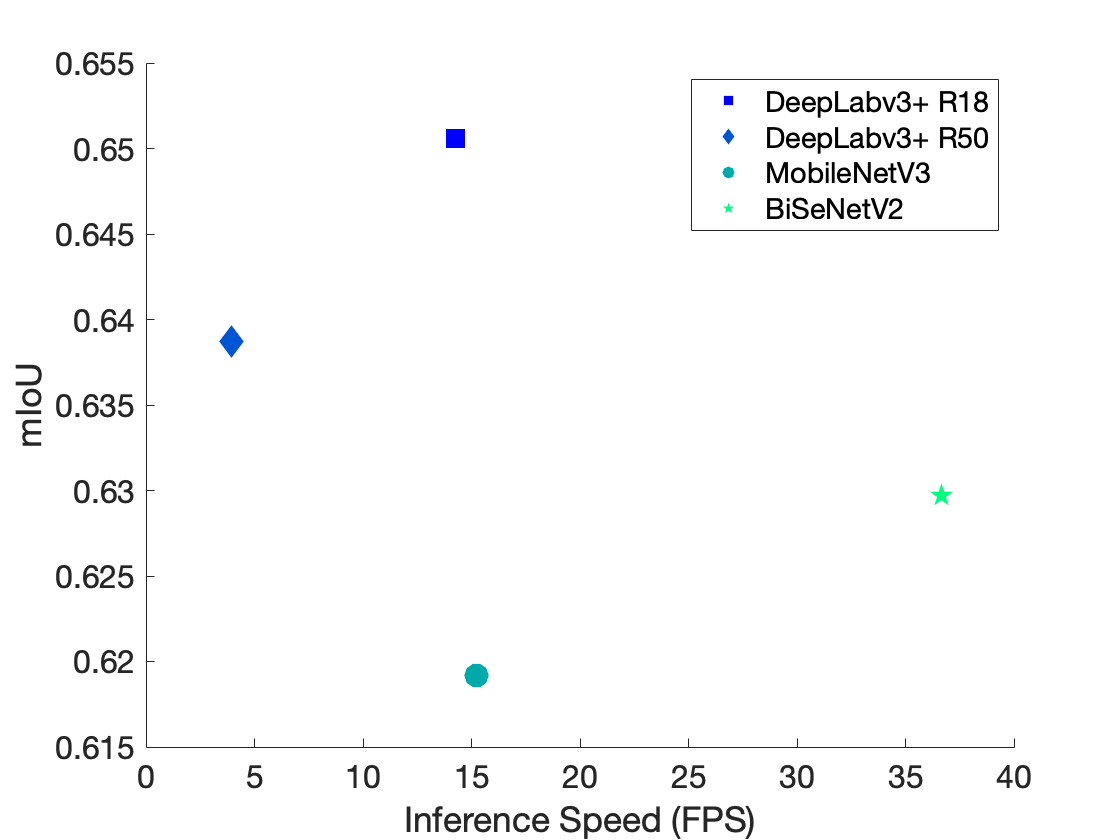
\includegraphics[width=0.75\columnwidth]{figure/pqe/Trade-off.png}
    \caption{The trade-off evaluation between inference speed and segmentation mean Intersection over Union (mIoU) for state-of-the-art segmentation network\cite{yu2021bisenet,howard2019searching,chen2018encoder} }
    \label{cross-evaluation}
 \end{figure}

 \begin{figure}[!ht]
    \centering
    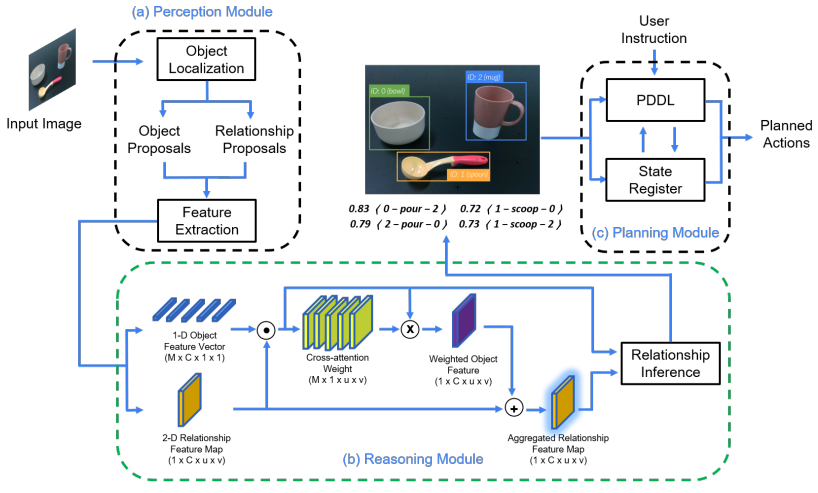
\includegraphics[width=0.9\columnwidth]{figure/pqe/pipeline_relationship.png}
    \caption{The whole pipeline of relationship-oriented semantic scene understanding. Overview: the pipeline first uses (a) perception module to localize all possible object and relationship proposals. A novel relationship-attention
    the mechanism in the (b) reasoning module is then deployed to aggregate the relationship feature map and infer the relationships along with their probabilities.
    Finally, the output from the last step seeds the (c) planning module for goal-oriented, multi-step manipulation task planning according to user instructions. }
    \label{fig:pipeline_relationship}
 \end{figure}

 \begin{figure}[!ht]
    \centering
    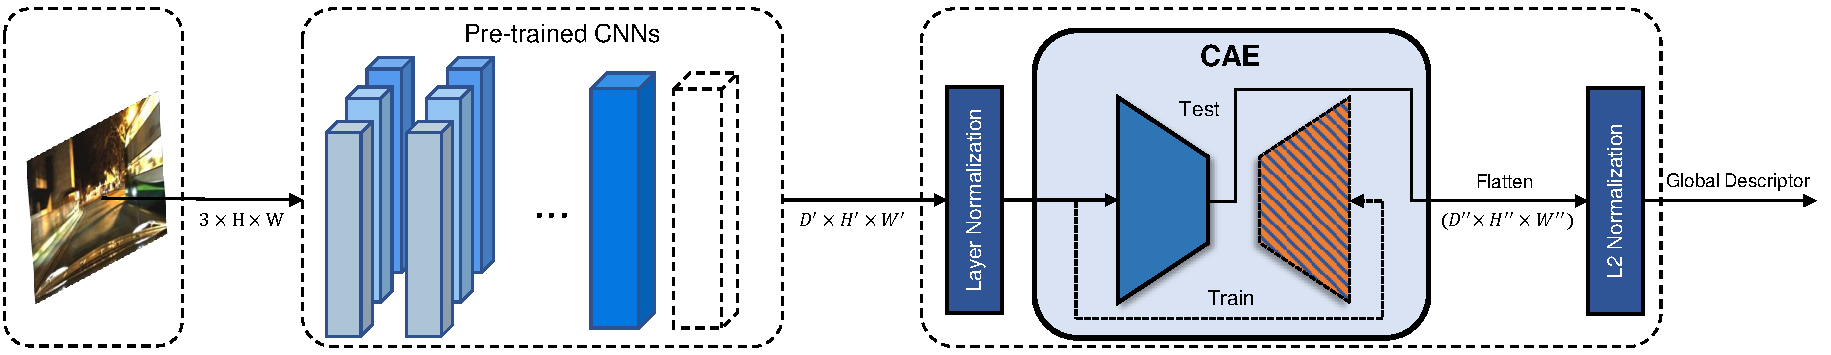
\includegraphics[width=\columnwidth]{figure/pqe/approach.pdf}
	\caption{The detailed pipeline of \cite{ye2022condition}. Given an image with $3\times{H}\times{W}$, CNNs  extract the local feature map $X_i$ with $D^{'}\times{H^{'}}\times{W^{'}}$. The CNNs are classification pre-trained or VPR-trained, e.g. AlexNet, VGG16. Both are cut at the last convolutional layer (conv5), before ReLU. In the training time, CAE is trained unsupervised by a reconstruction loss. In the test time, the decoder part of CAE is not involved and the encoder part is kept to compress the normalized feature map and produce a low-dimensional global descriptor with $D^{''}\times{H^{''}}\times{W^{''}}$. The global descriptor is then flattened and L2 normalized.}
    \label{fig:approach_VPR}
 \end{figure}



\begin{figure}[!ht]
\centering
\begin{subfigure}{0.4\textwidth}
    \centering
    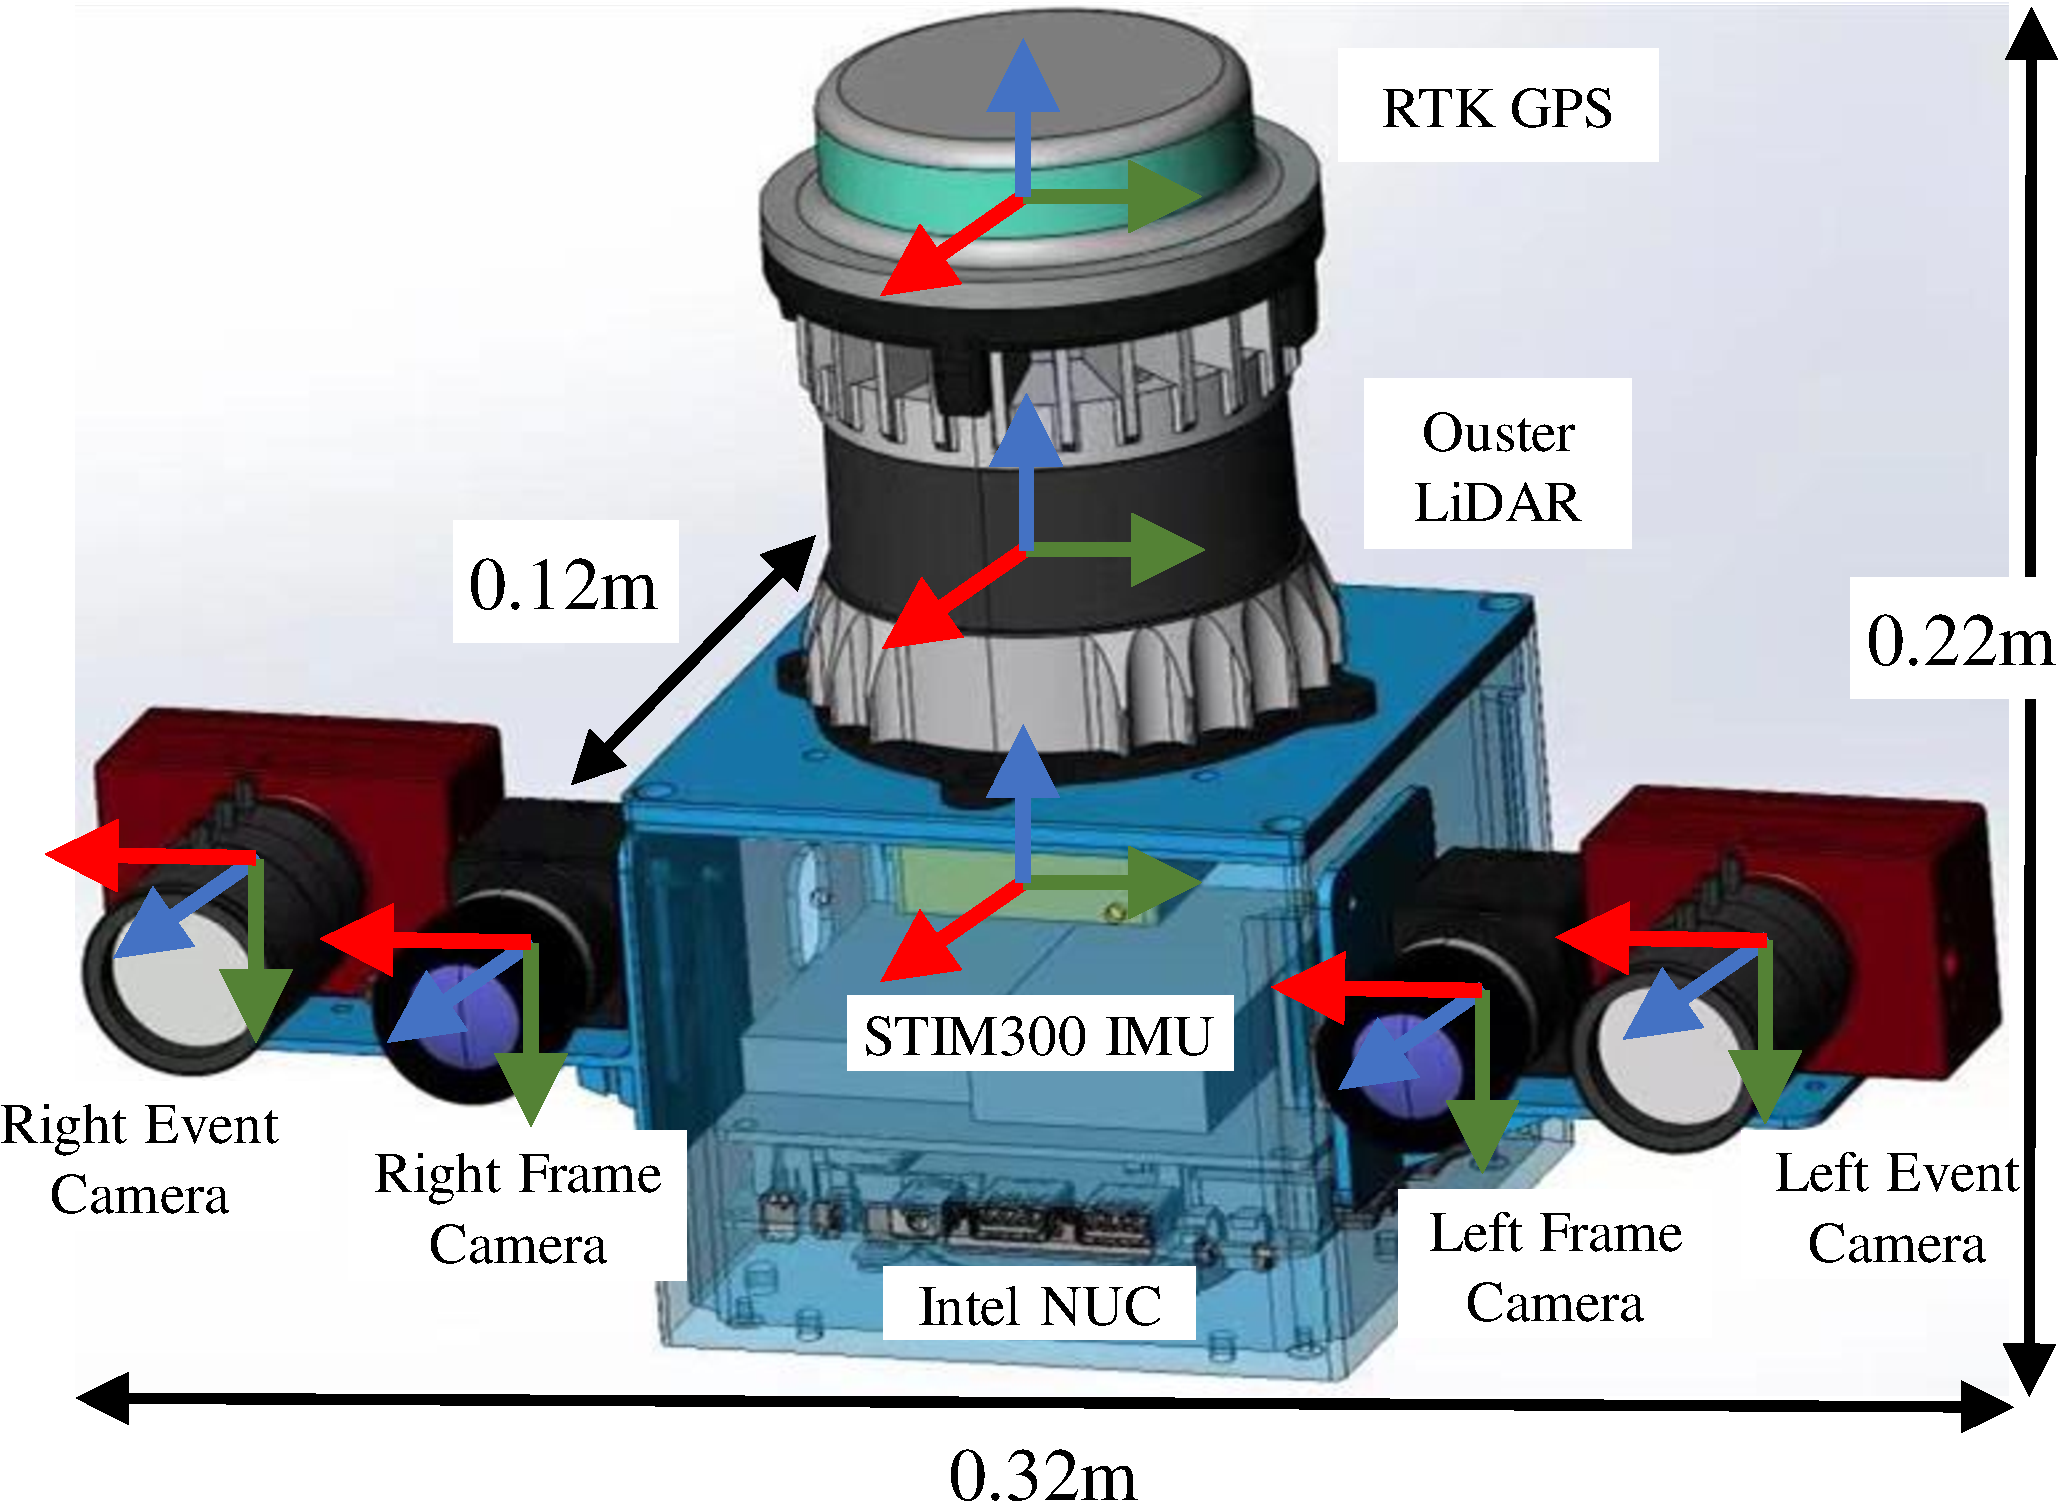
\includegraphics[width=0.8\textwidth, height=5cm]{figure/pqe/methodology/handheld_device-crop.pdf}
    \caption{}
    % \caption{A point cloud map of the second floor, HKUST CYT constructed by A-LOAM}
\end{subfigure}
\centering
\begin{subfigure}{0.4\textwidth}
    \centering
    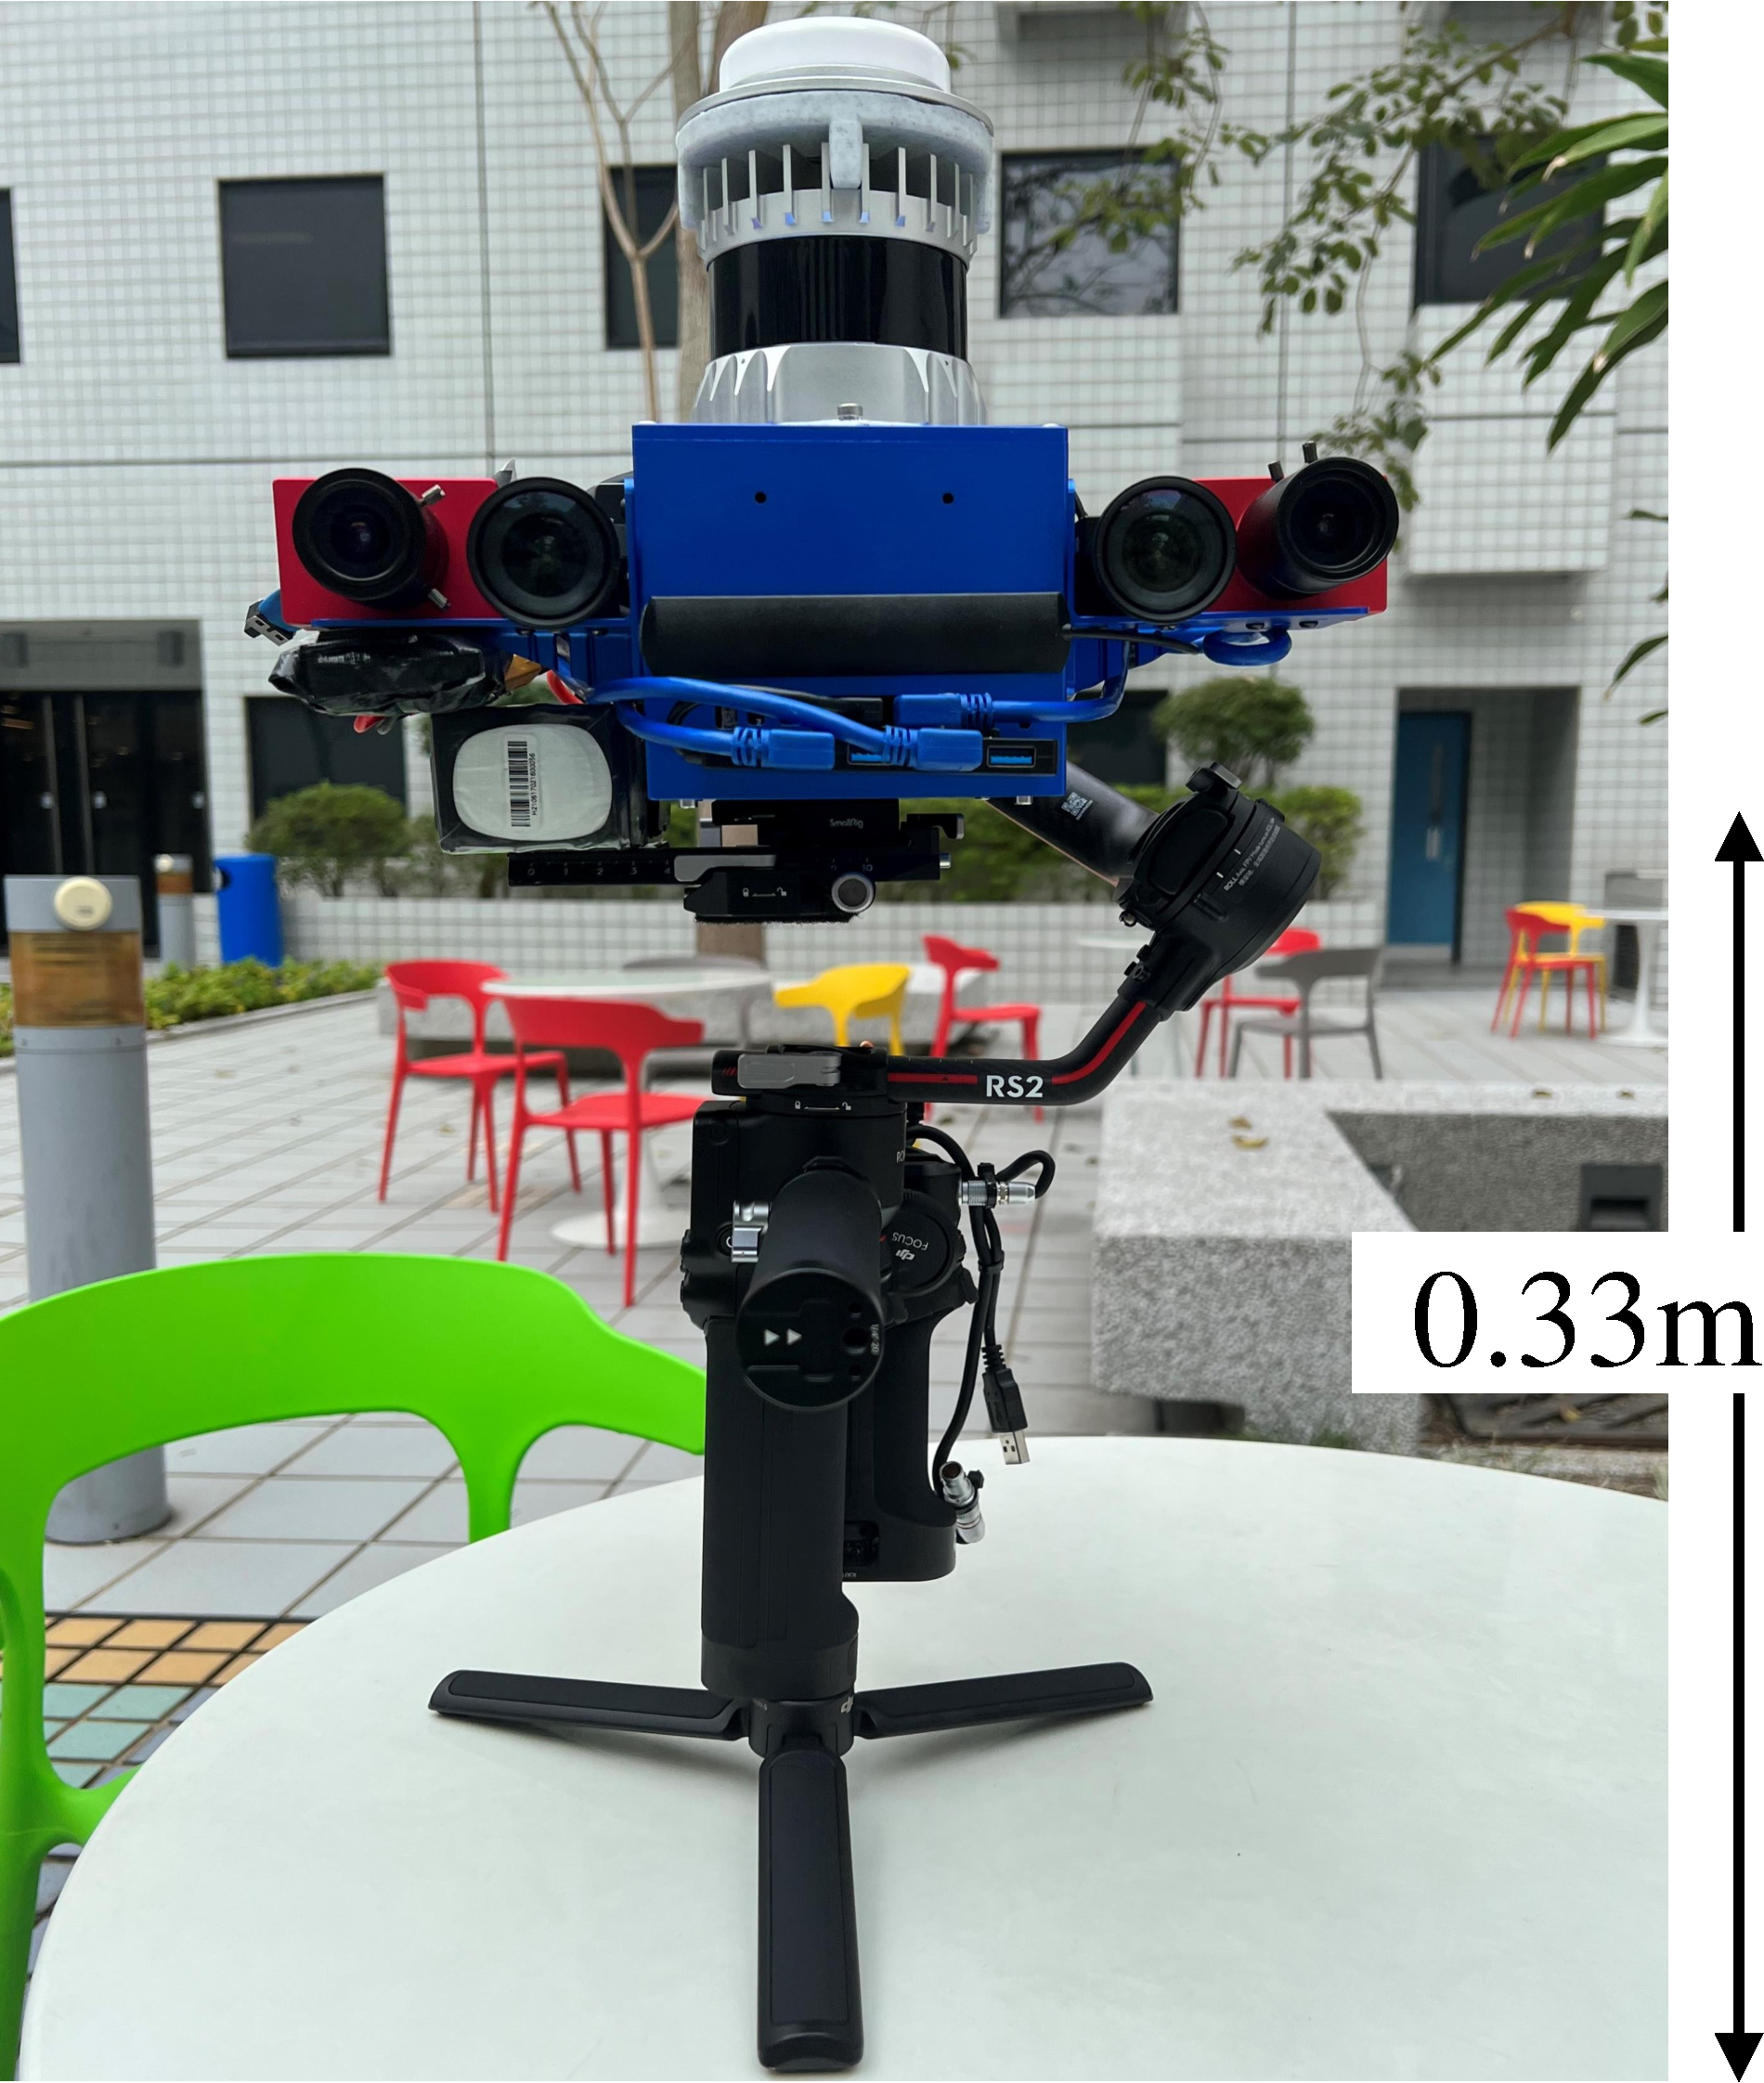
\includegraphics[width=0.8\textwidth, height=5cm]{figure/pqe/methodology/handheld_2-crop.pdf}
    \caption{}
    % \caption{A capture of localization on quadruped robot in an indoor office environment.}
\end{subfigure}
\begin{subfigure}{0.4\textwidth}
    \centering
    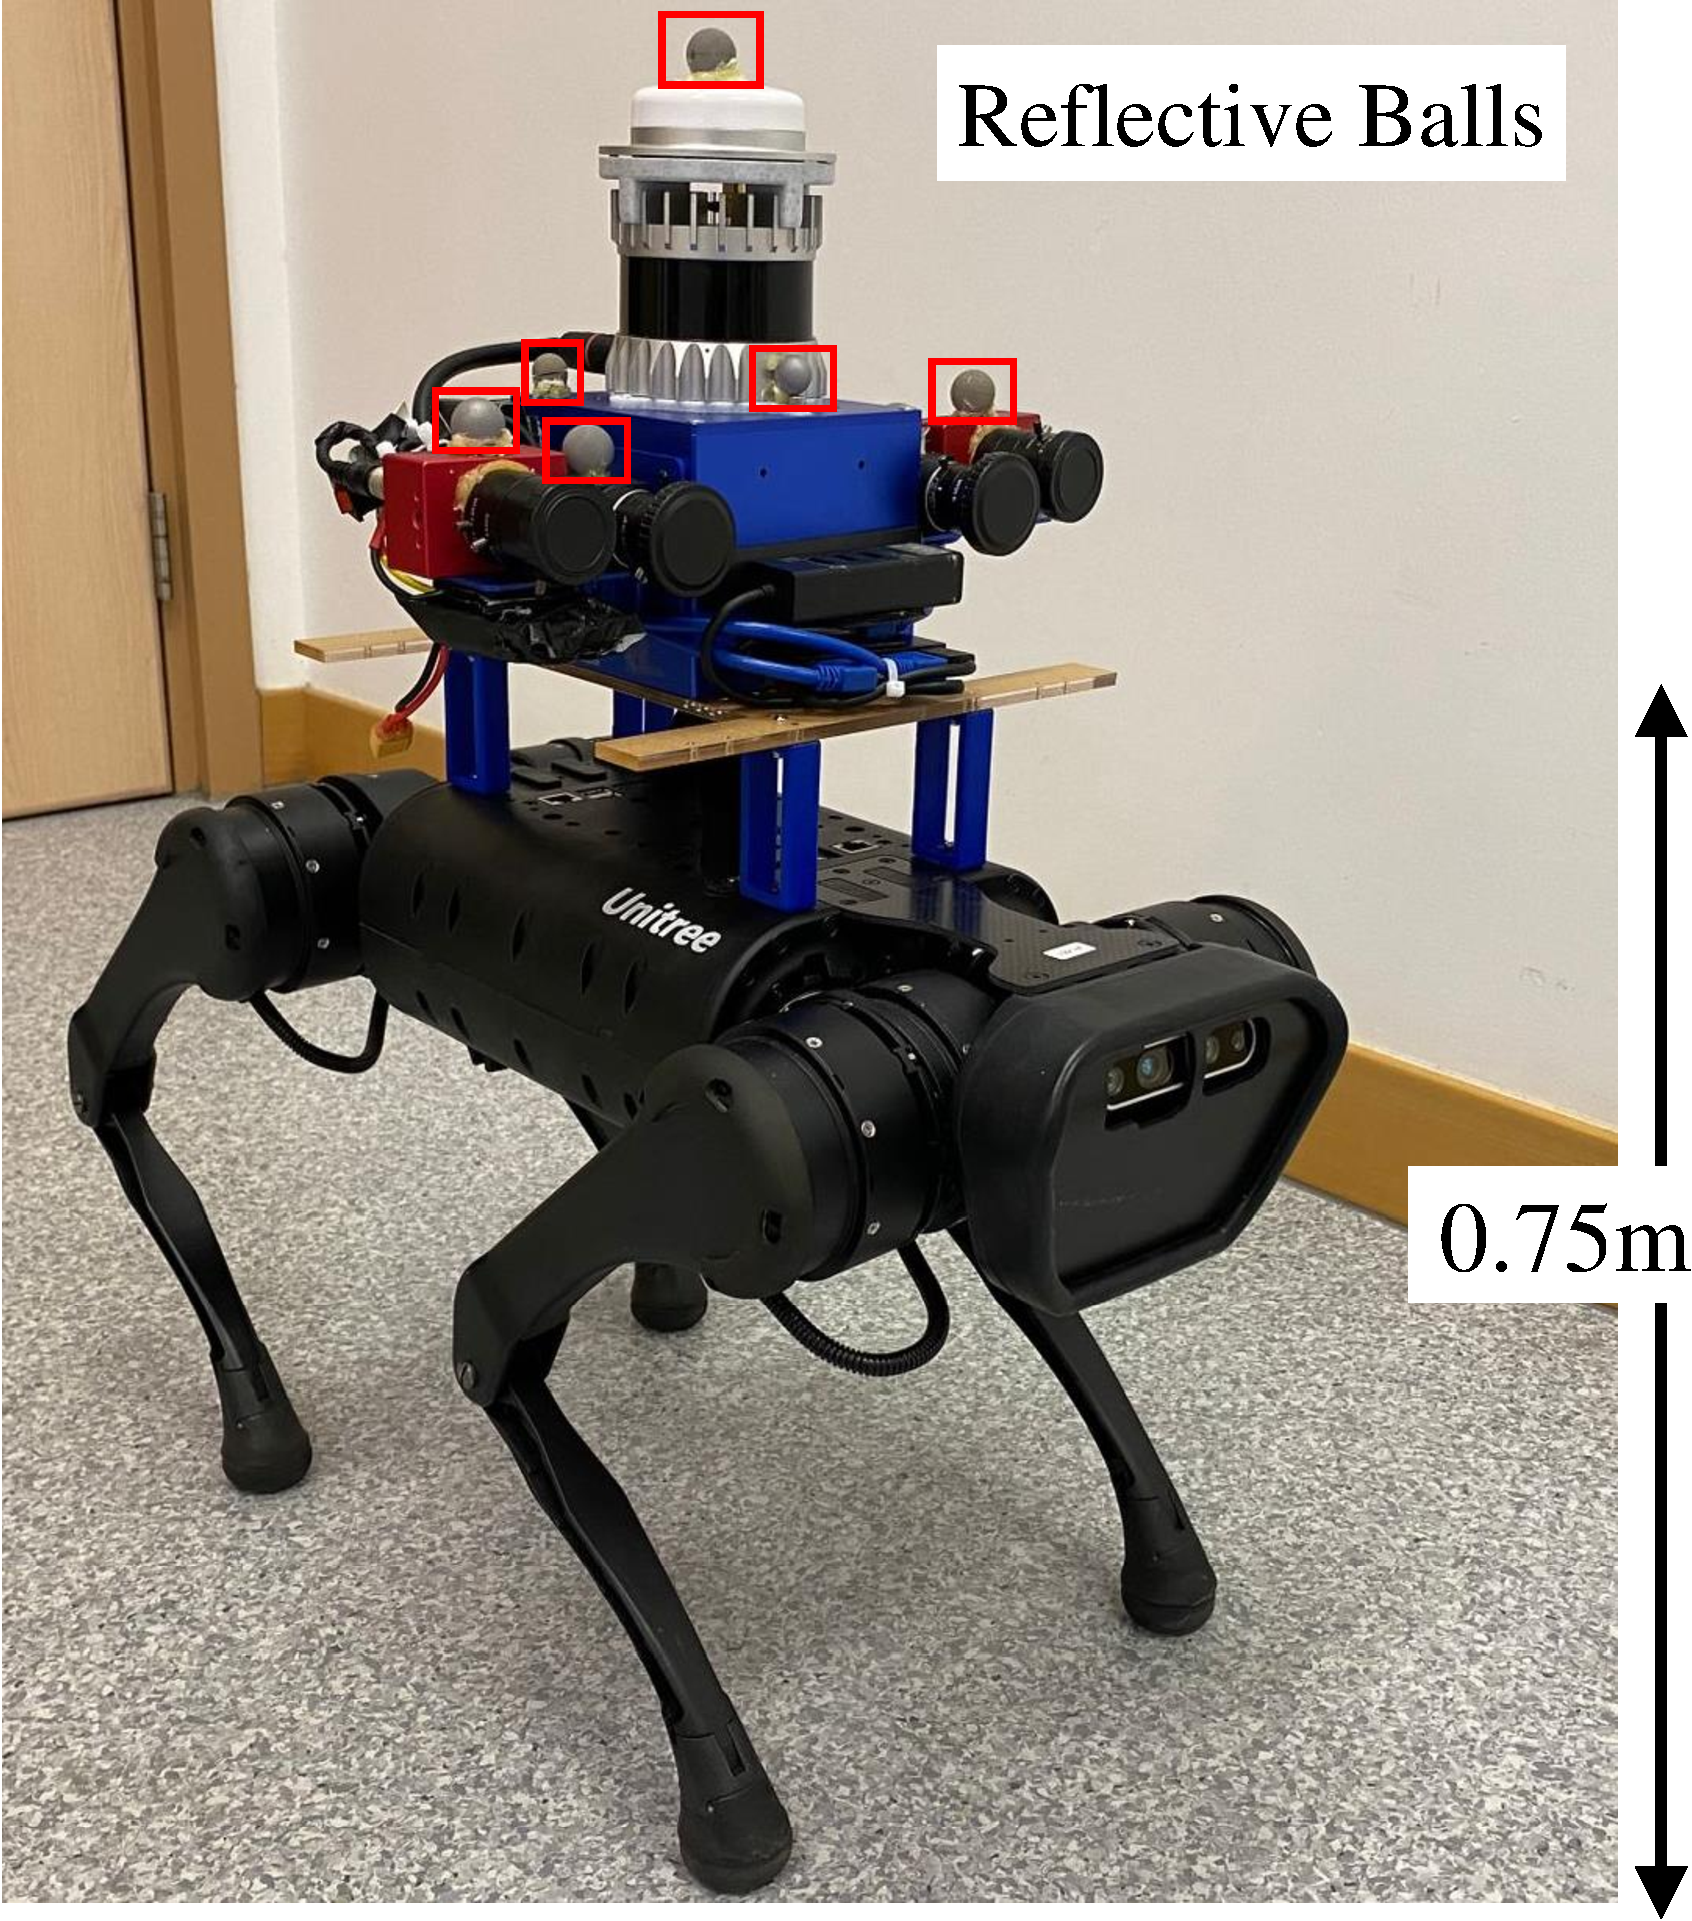
\includegraphics[width=0.8\textwidth, height=5cm]{figure/pqe/methodology/robotdog-crop.pdf}
    \caption{}
    % \caption{A capture of localization on quadruped robot in an indoor office environment.}
\end{subfigure}
\begin{subfigure}{0.4\textwidth}
    \centering
    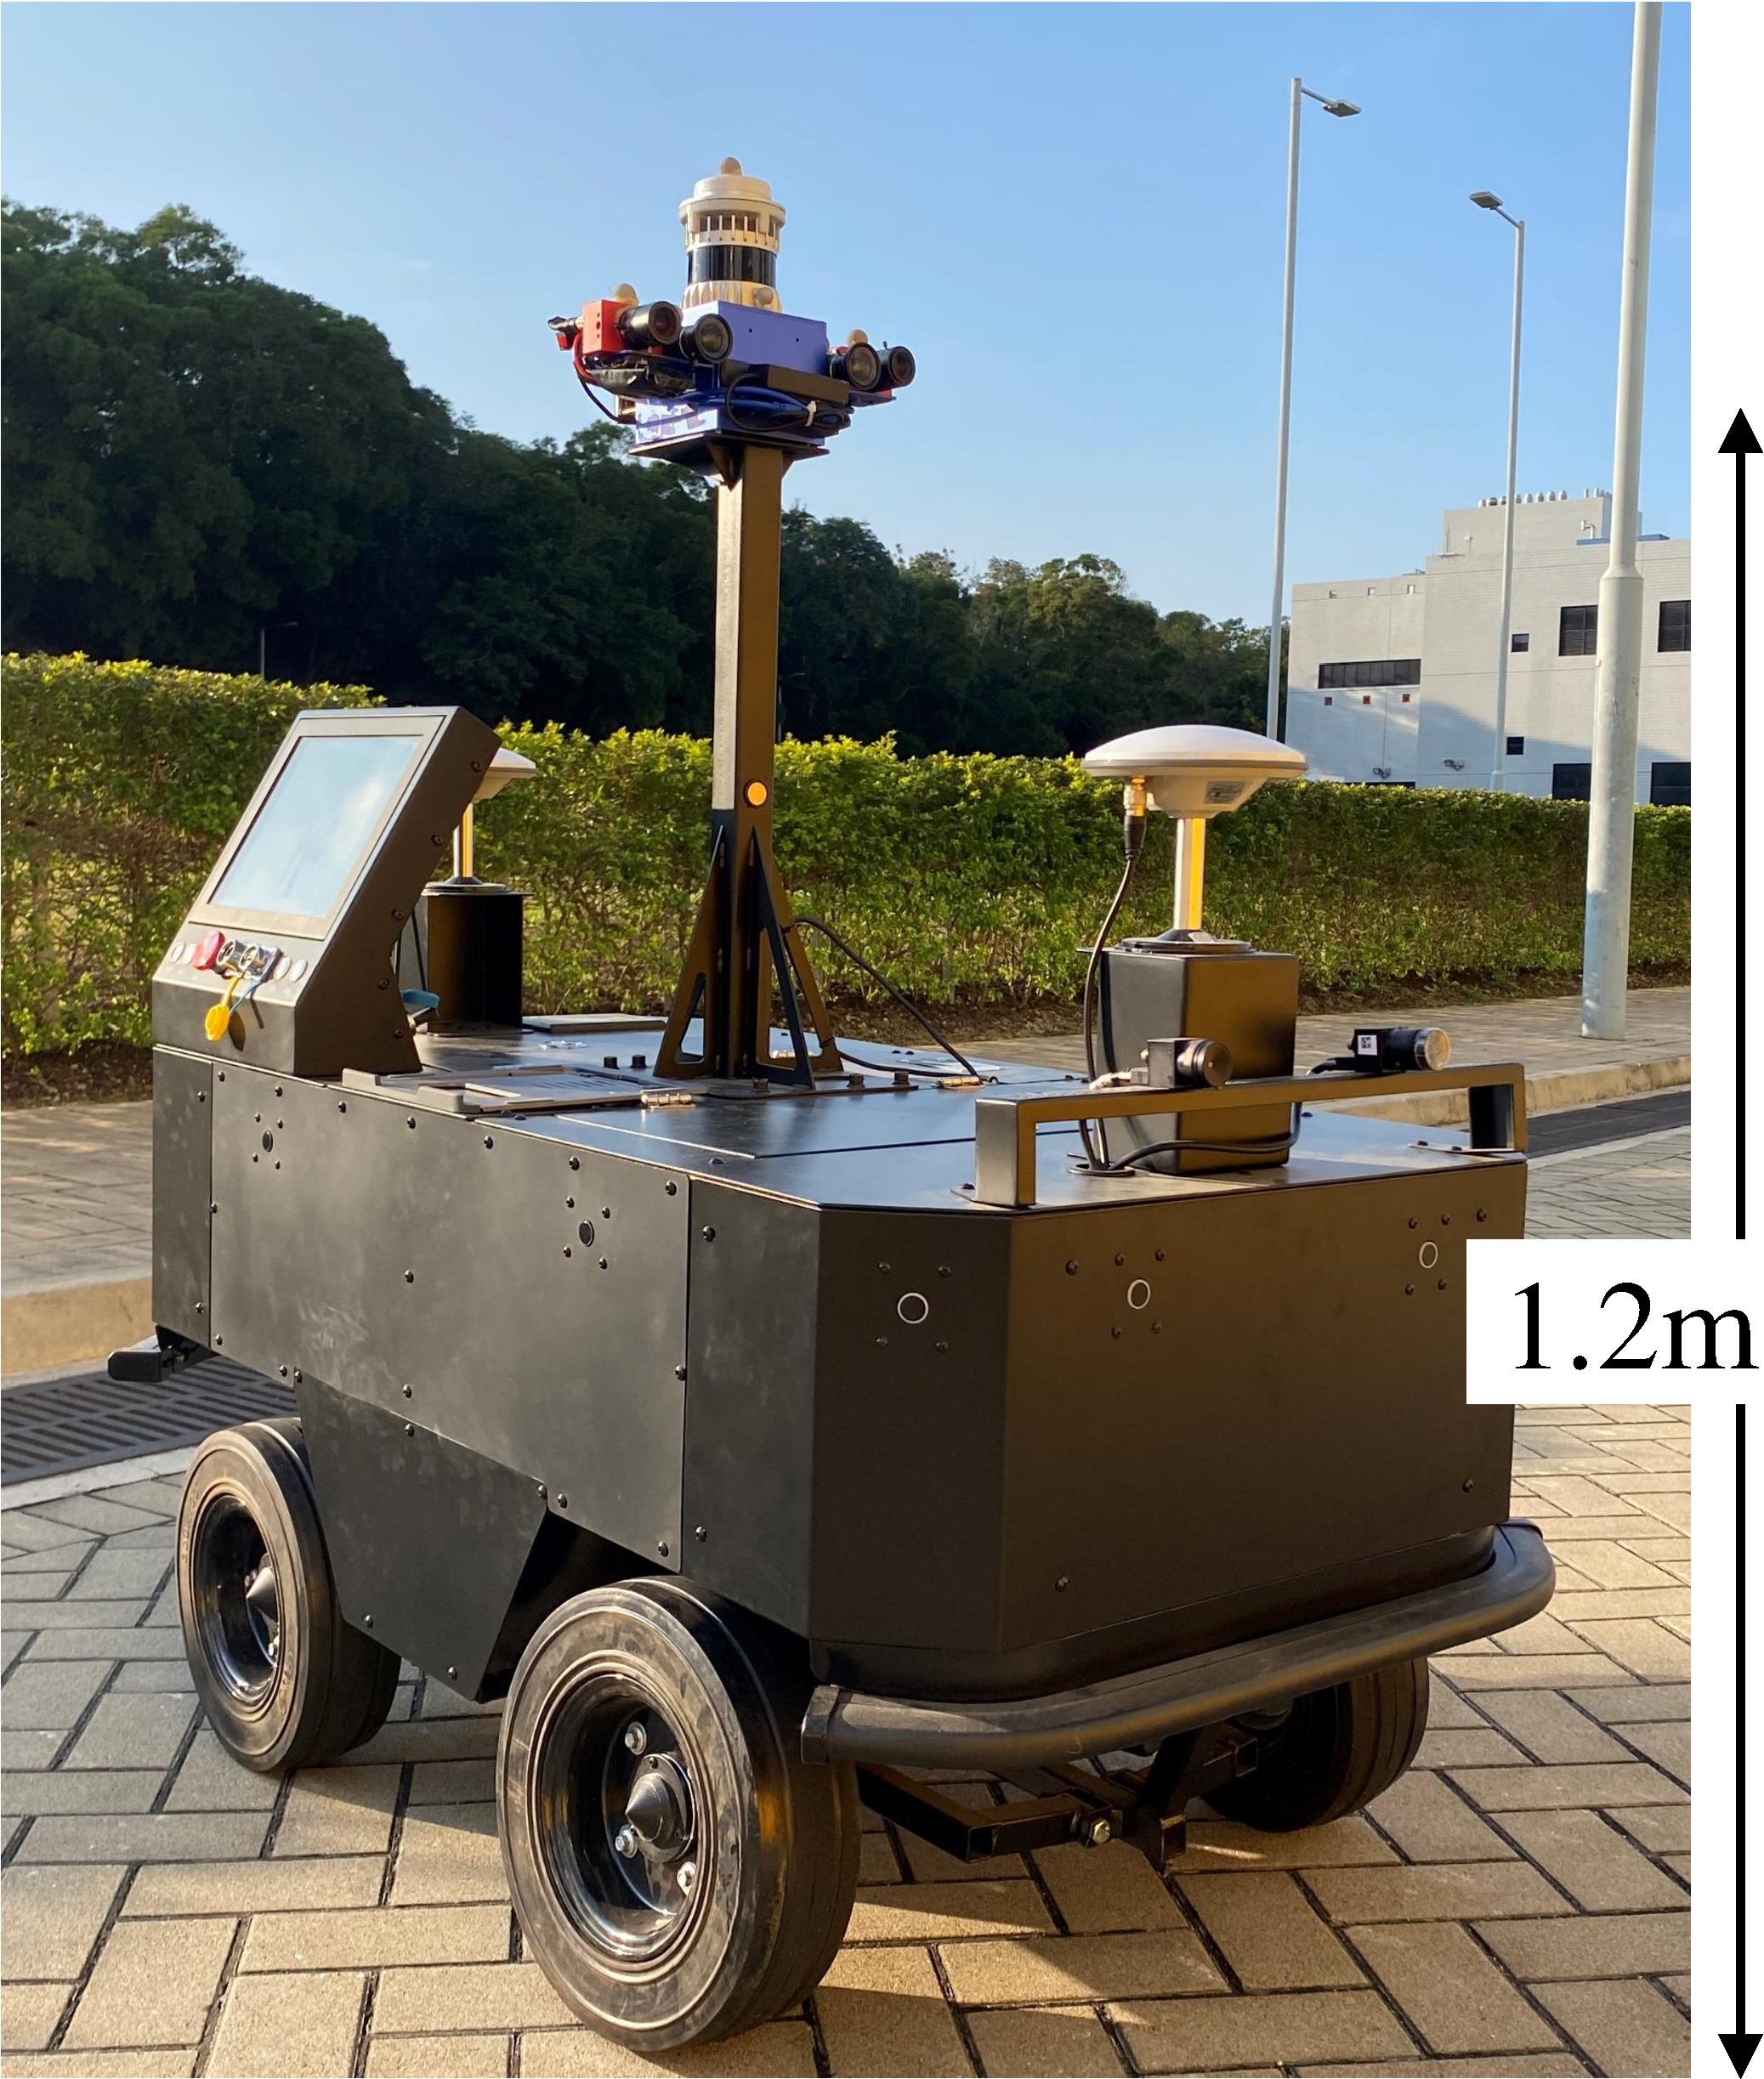
\includegraphics[width=0.8\textwidth, height=5cm]{figure/pqe/methodology/apollo-crop.pdf}
    \caption{}
    % \caption{A capture of localization on quadruped robot in an indoor office environment.}
\end{subfigure}

\caption{The multi-sensor device and data collection platform: 
(a) CAD model of the sensor rig, where axis directions are colored: red: $X$, green: $Y$, blue: $Z$. The sensor rig is rigidly mounted on (b) a gimbal stabilizer, (c) a quadruped robot, and (d) an apollo autonomous vehicle.}
\label{fig:FusionPortable}
\end{figure}
 
 



% \begin{figure}[ht]
% \centering
% \begin{subfigure}
% {\label{fig:sensor_handheld}
% \hspace{0.2cm}
% \centering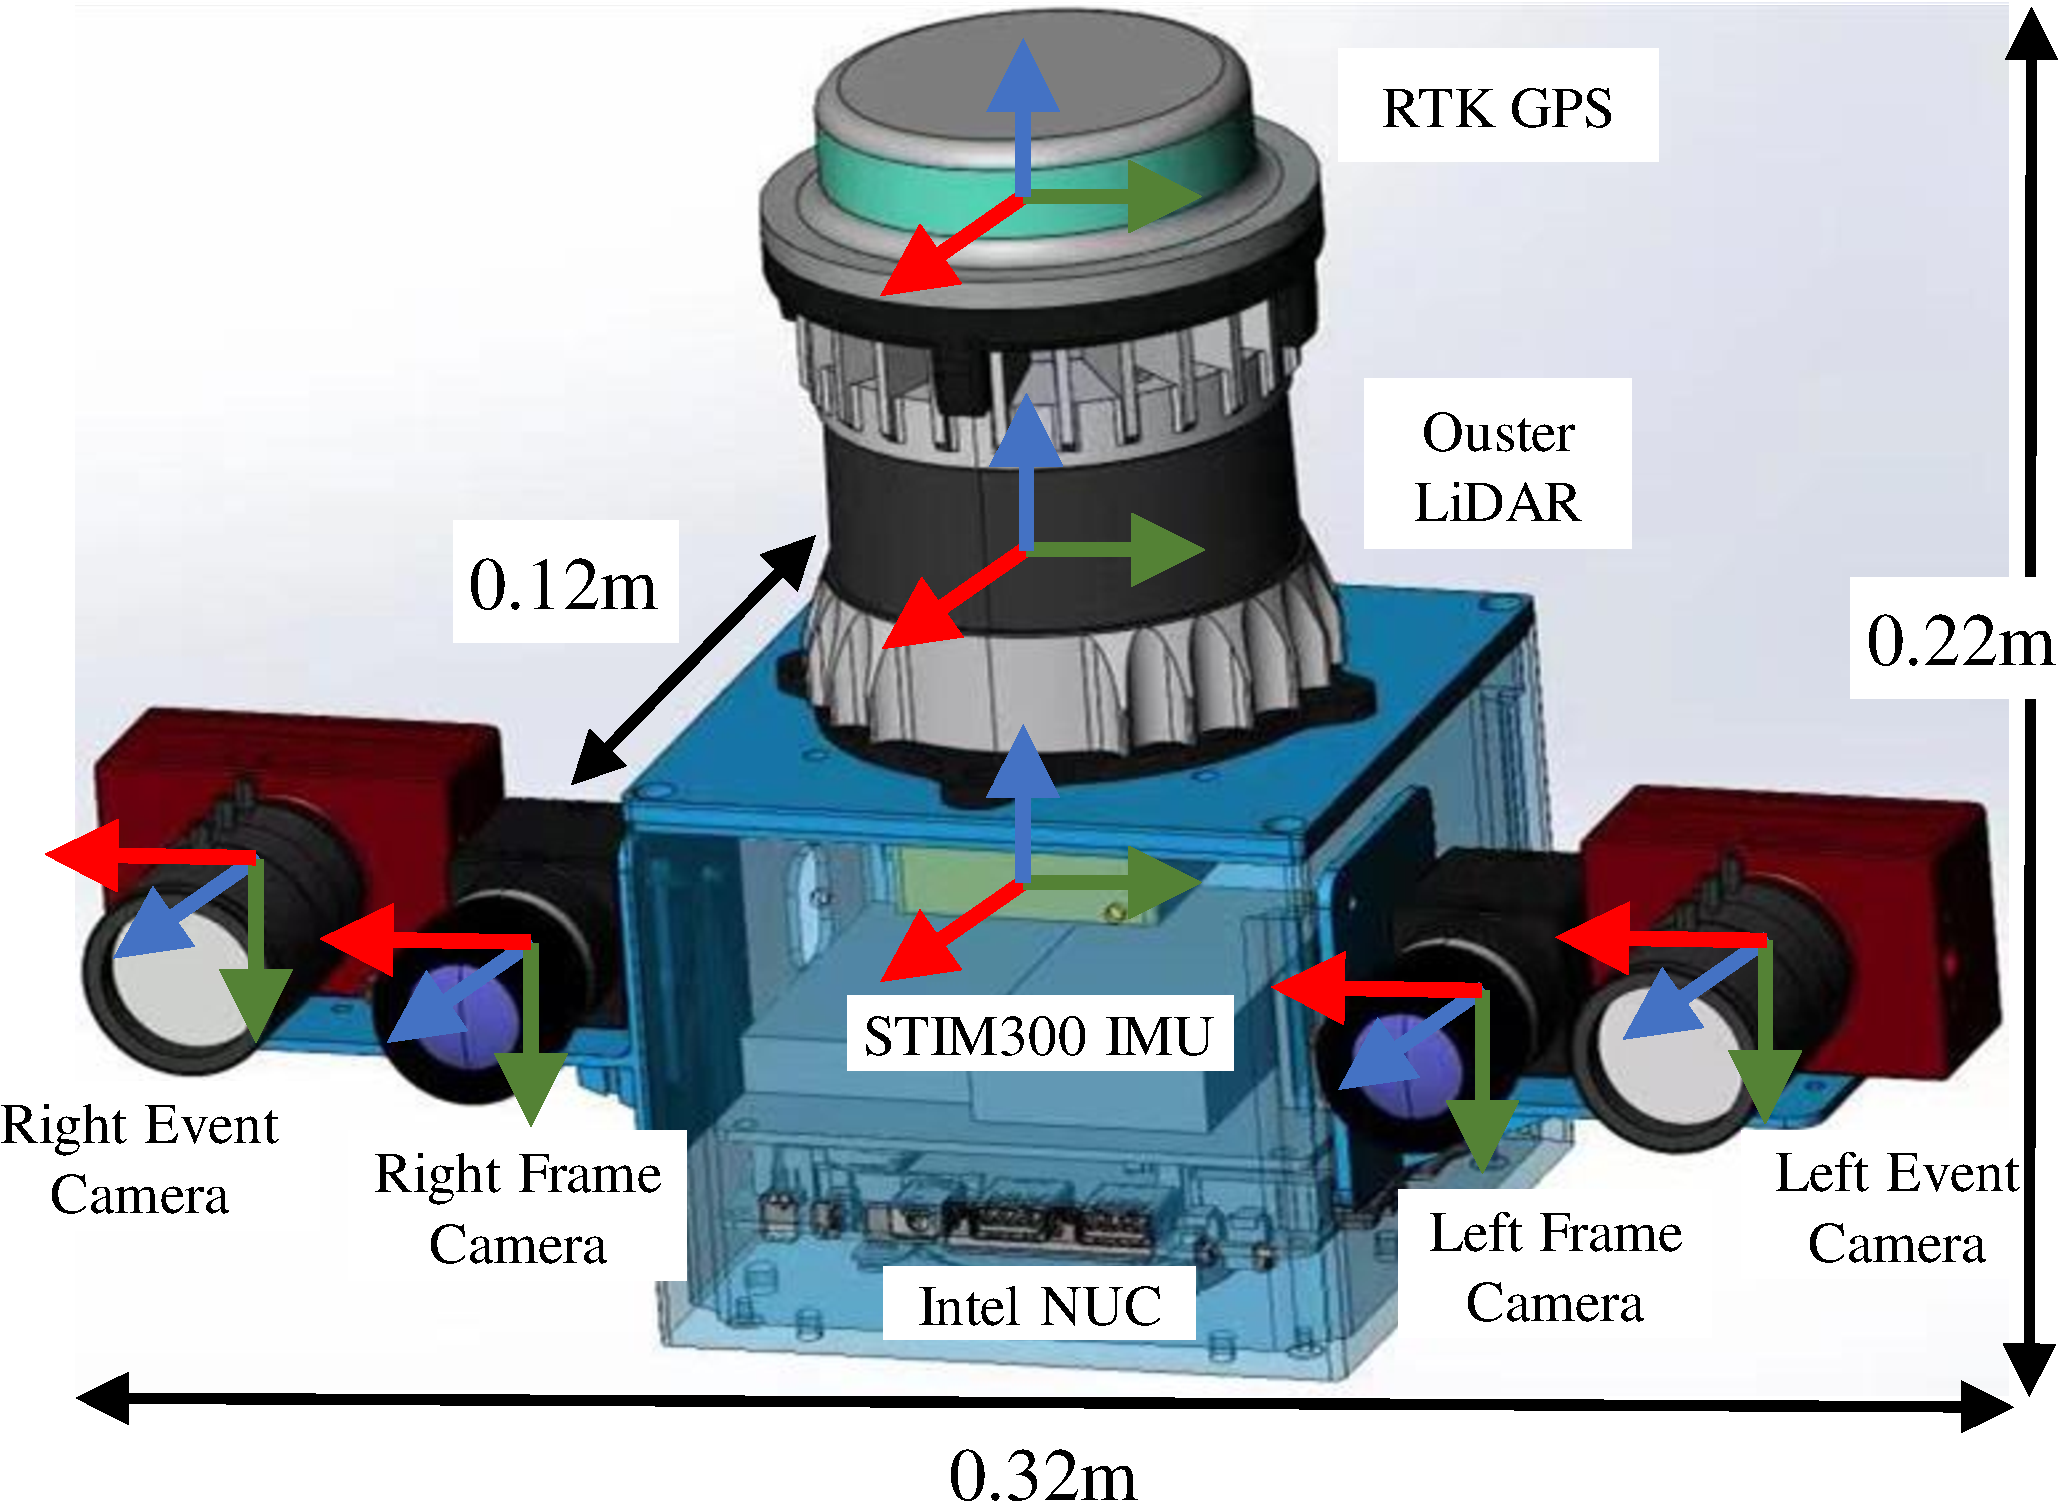
\includegraphics[width=.2746\linewidth]{figure/pqe/methodology/handheld_device-crop.pdf}}
% \end{subfigure}
% \begin{subfigure}{\label{fig:sensor_stab}\centering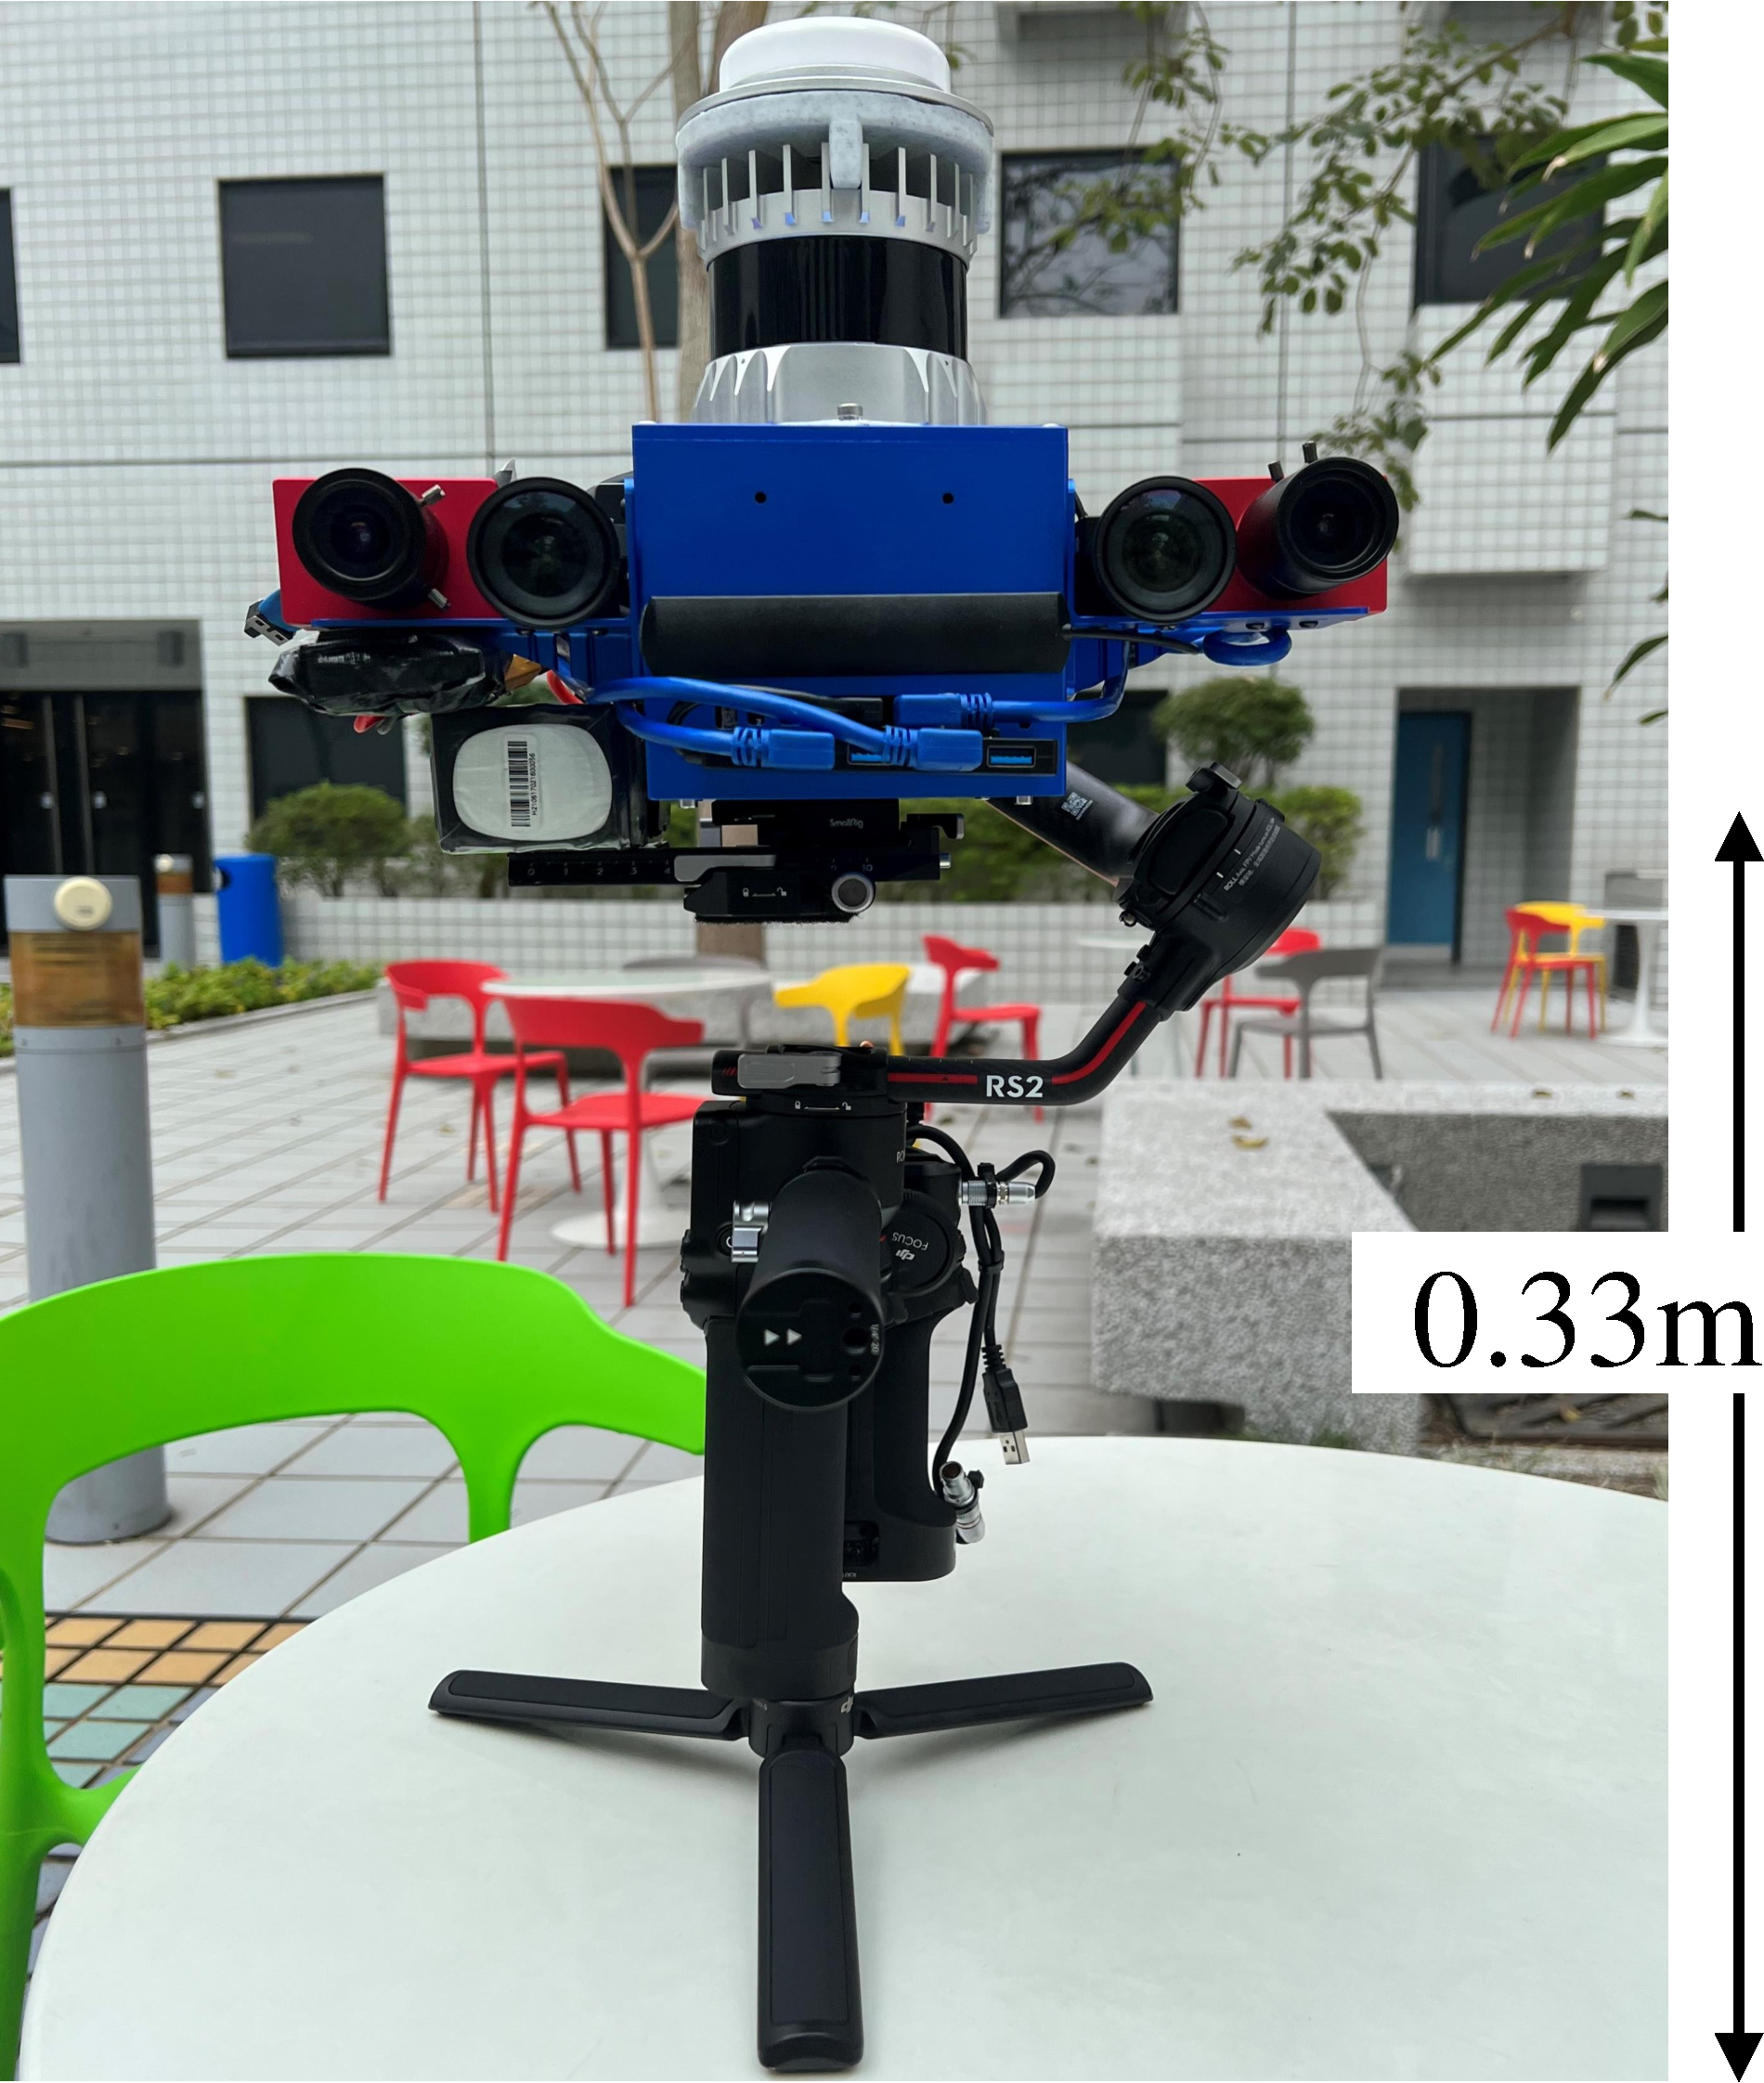
\includegraphics[width=.1701\linewidth]{figure/pqe/methodology/handheld_2-crop.pdf}}
% \end{subfigure}
% \begin{subfigure}{\label{fig:sensor_quadrobot}\centering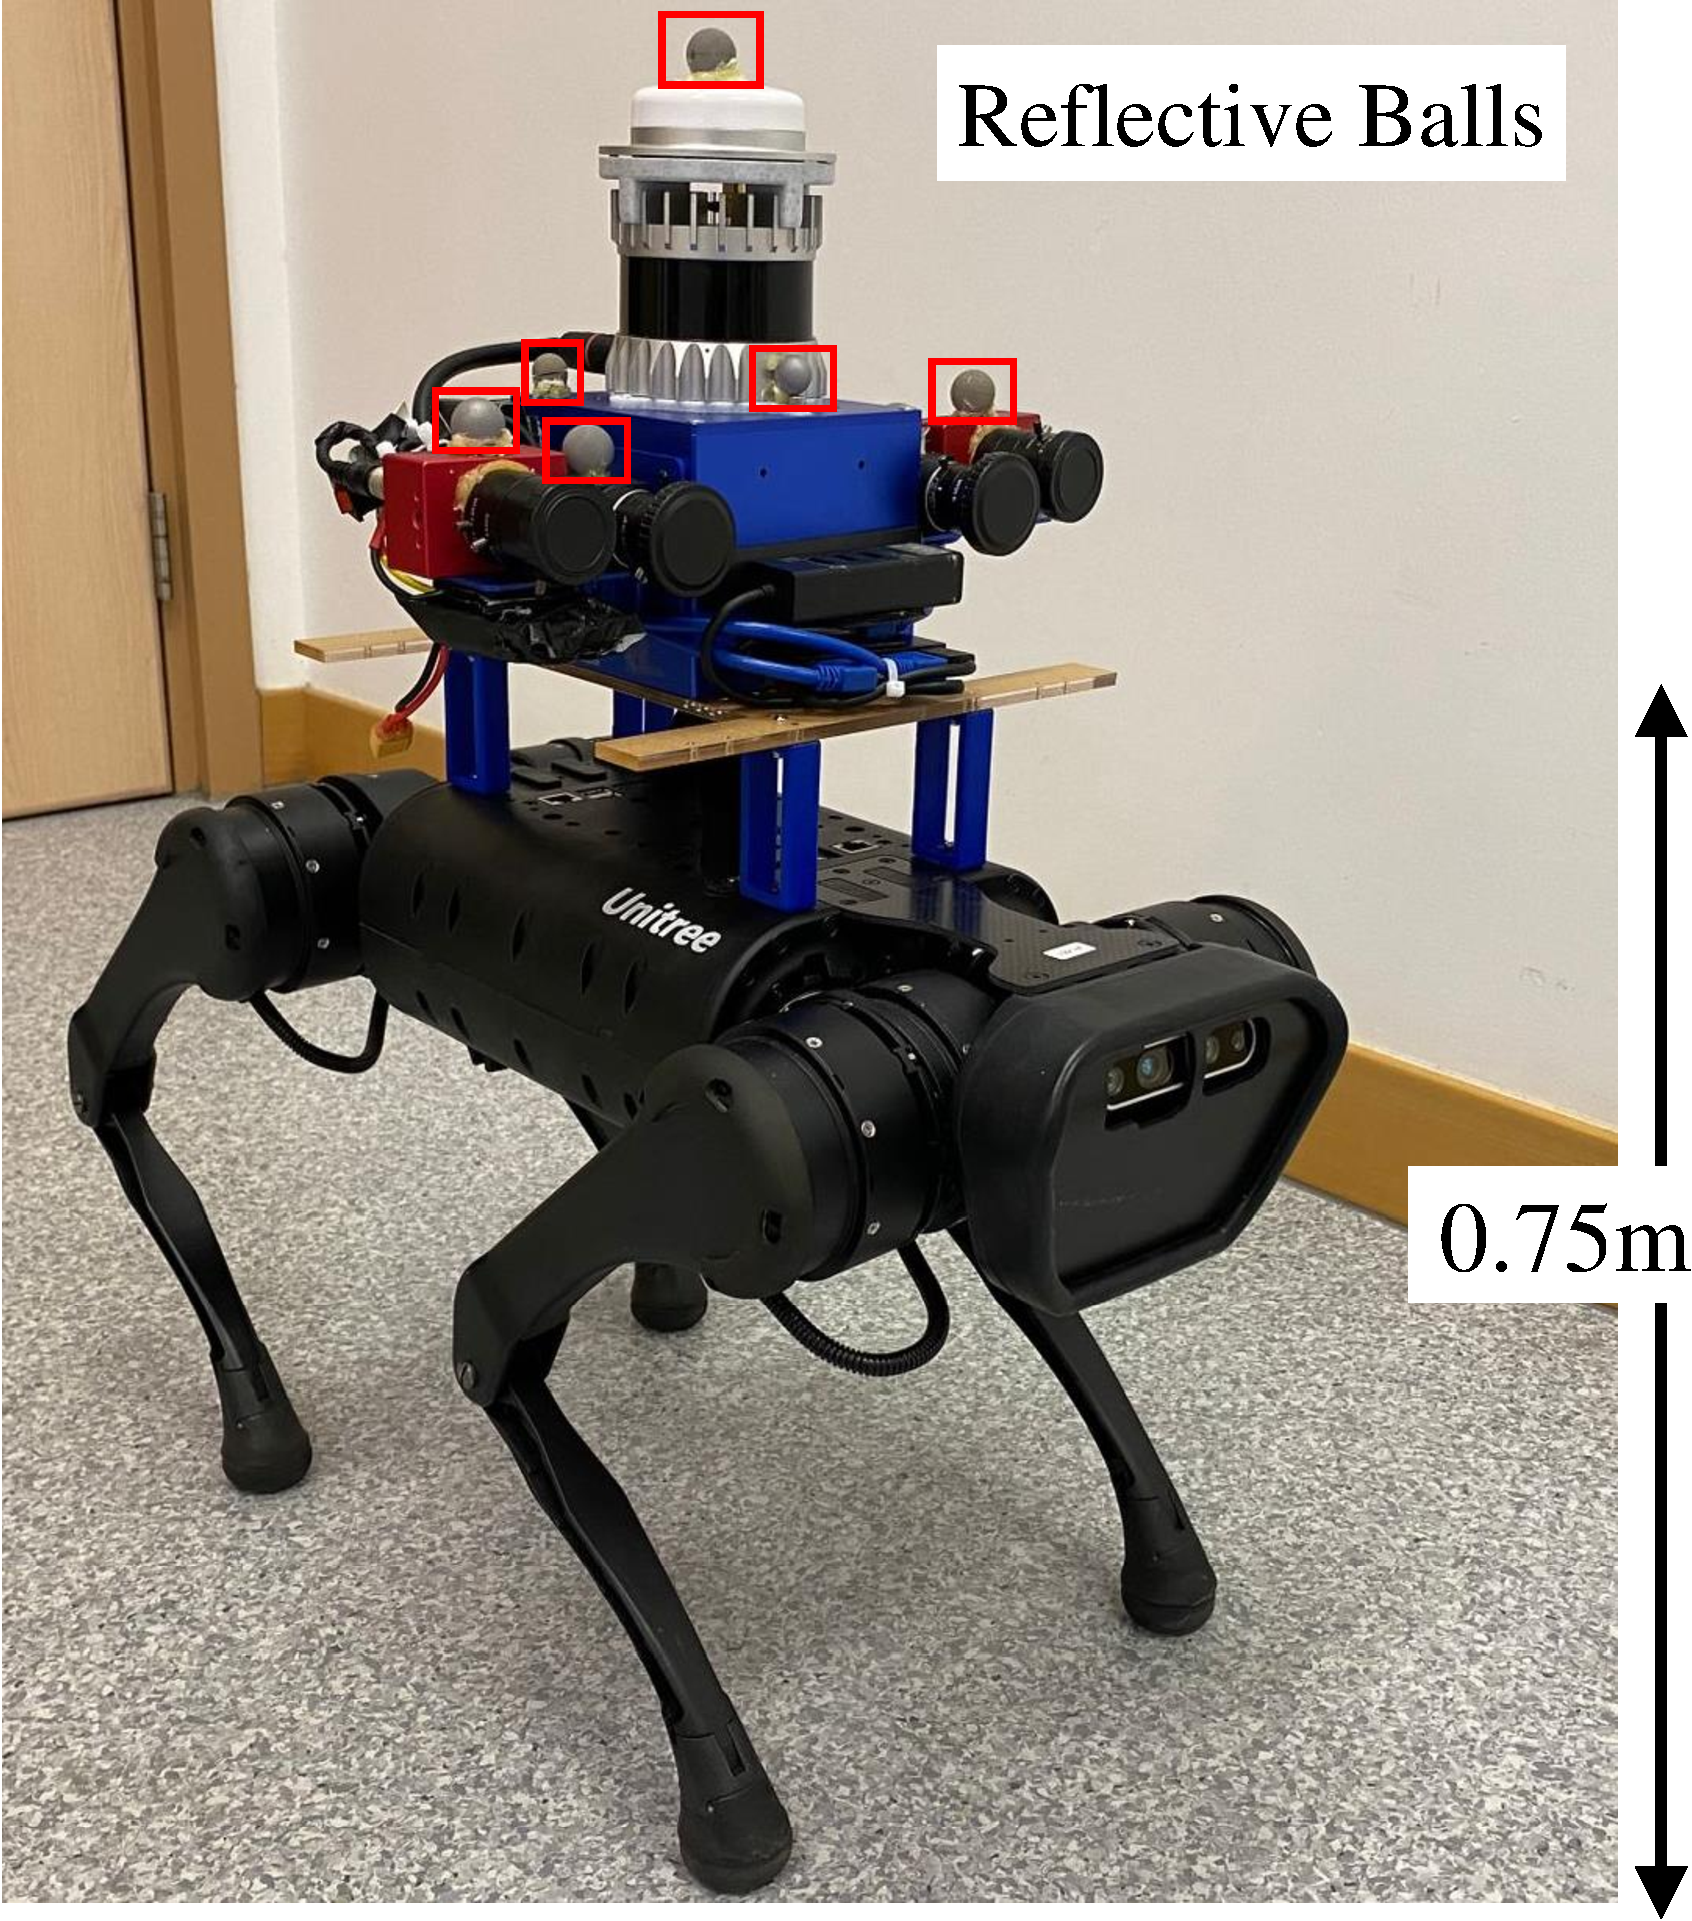
\includegraphics[width=.1776\linewidth]{figure/pqe/methodology/robotdog-crop.pdf}}
% \hspace{0.2cm}
% \end{subfigure}
% \begin{subfigure}
%     {\label{fig:sensor_apollo}\centering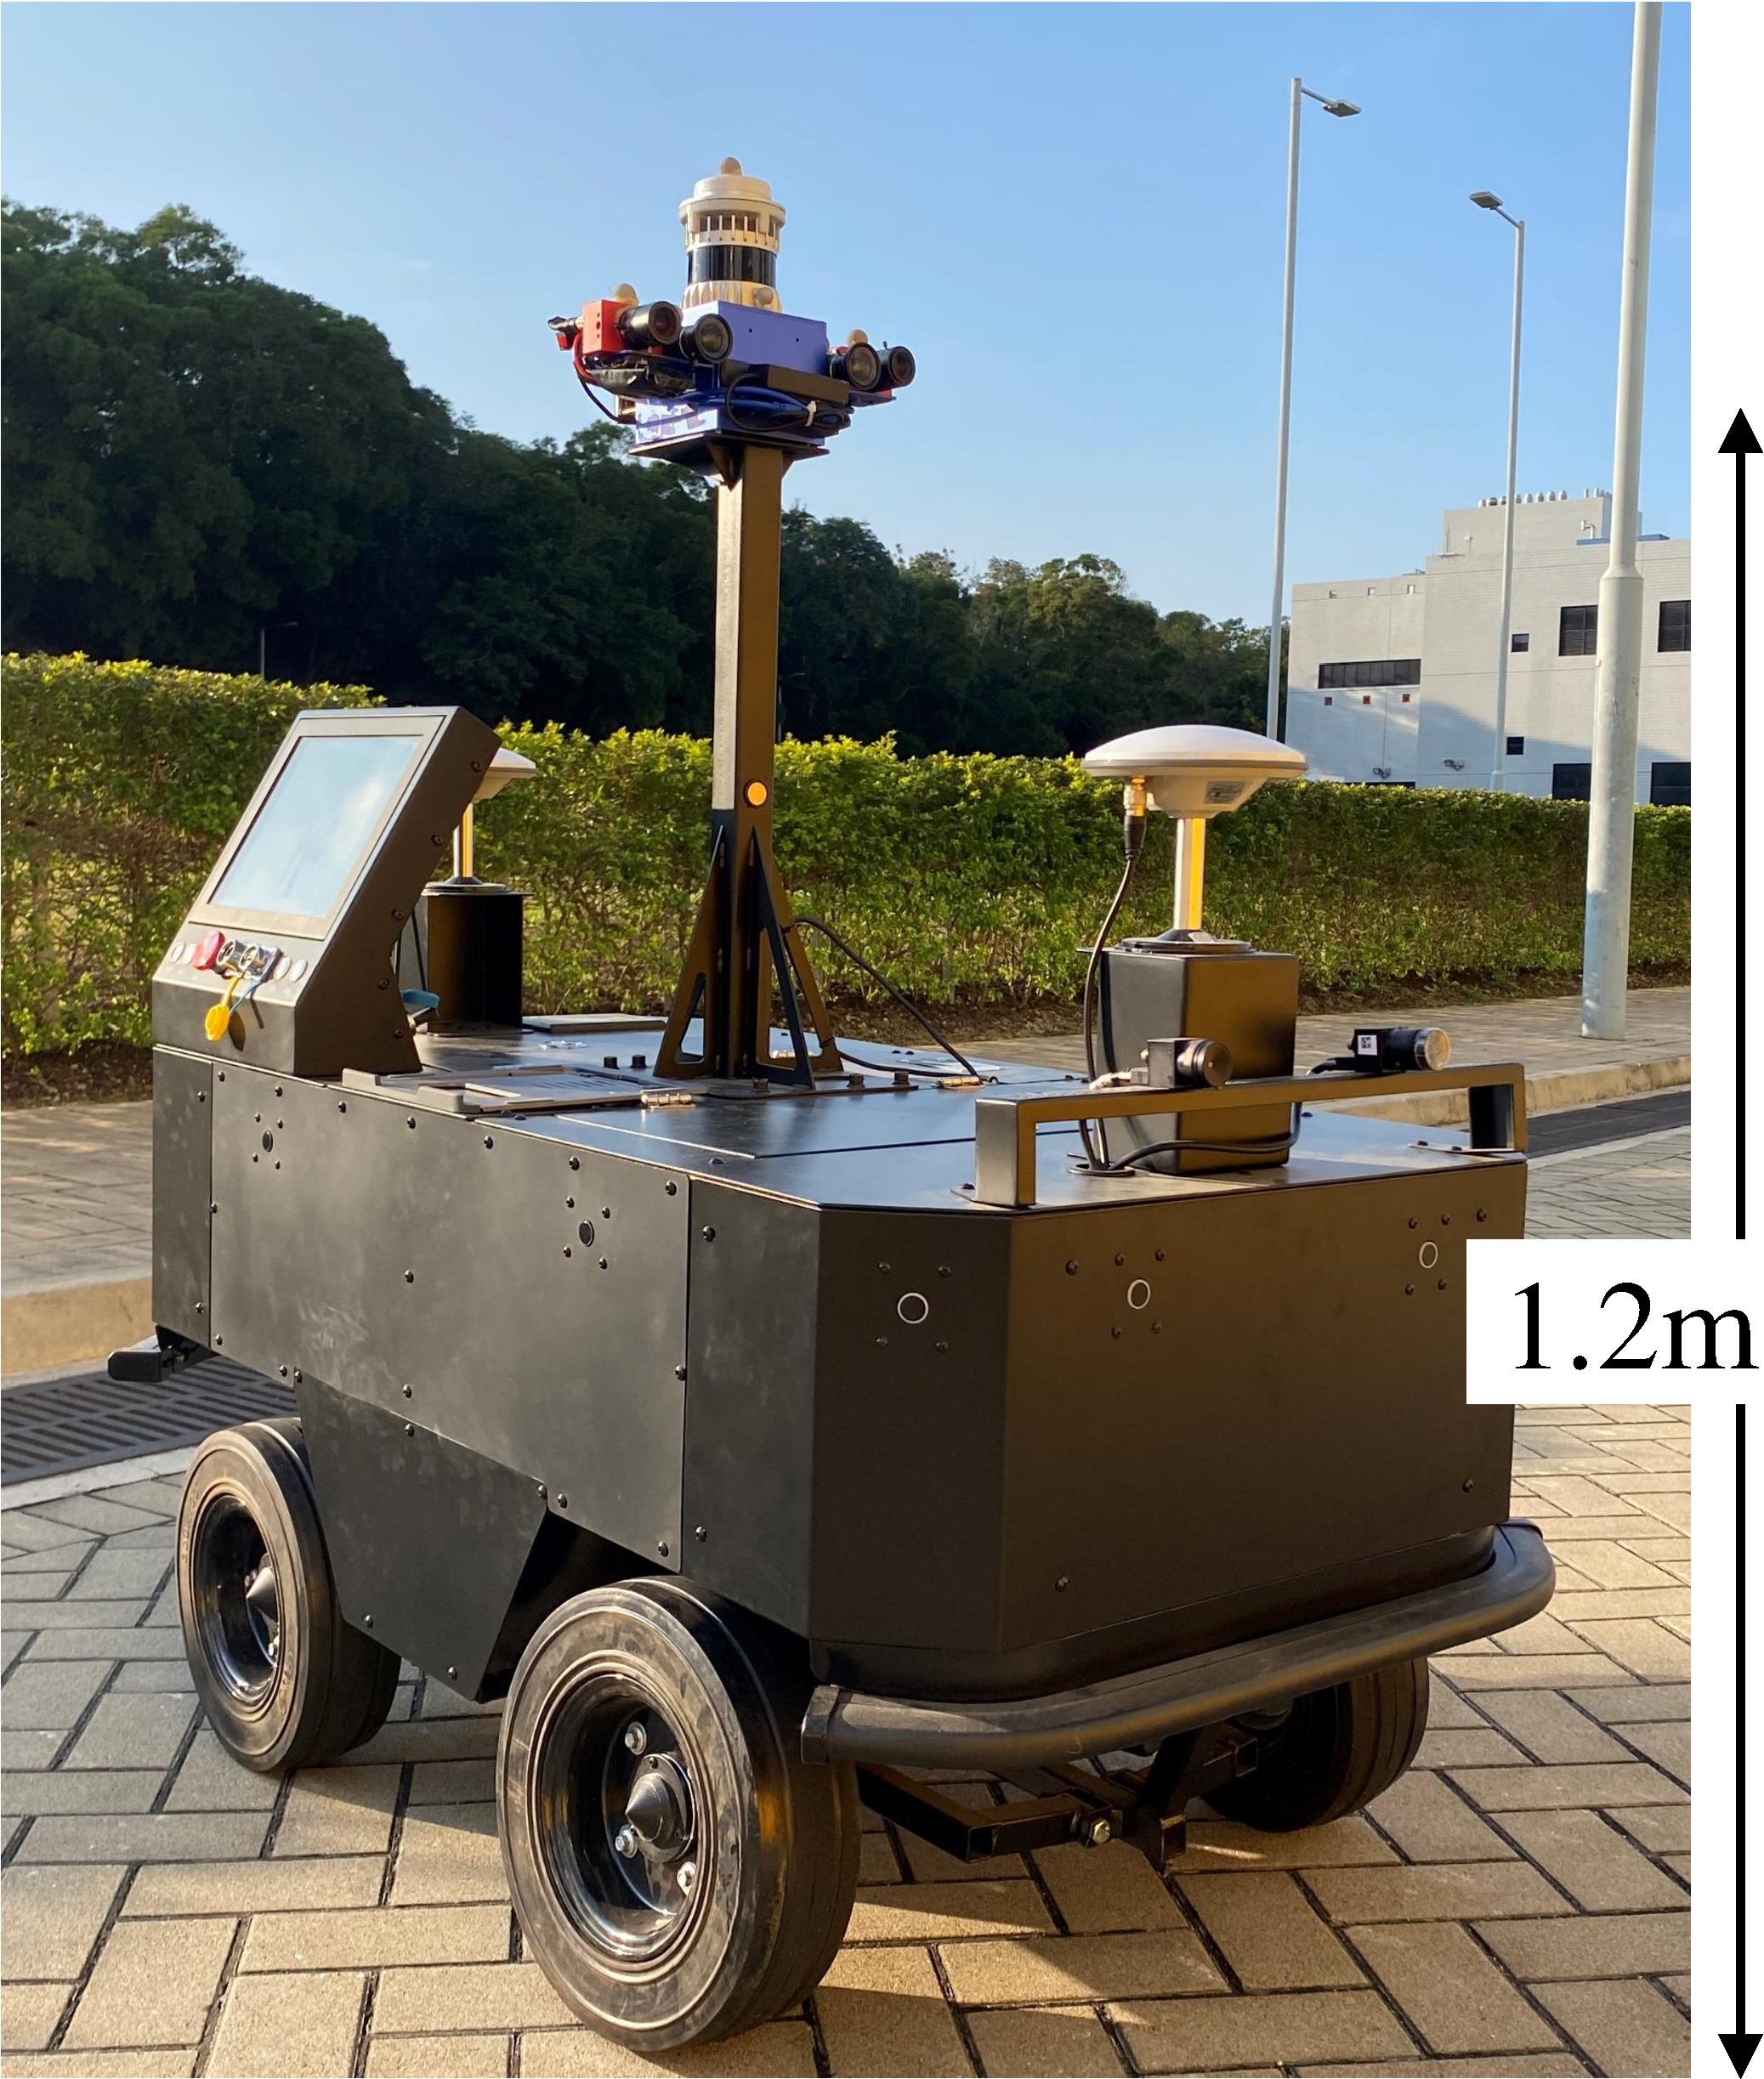
\includegraphics[width=.1701\linewidth]{figure/pqe/methodology/apollo-crop.pdf}} 
% \end{subfigure}
% \caption{The multi-sensor device and data collection platform: 
% (a) CAD model of the sensor rig, where axis directions are colored: red: $X$, green: $Y$, blue: $Z$. The sensor rig is rigidly mounted on (b) a gimbal stabilizer, (c) a quadruped robot, and (d) an apollo autonomous vehicle.}
% \label{fig:sensor_picture}
% \vspace{-0.3cm}
% \end{figure}  





